\documentclass[12pt,oneside]{report}
\usepackage[titletoc]{appendix}
\usepackage{setspace}
\usepackage{amsmath}
\usepackage[pdftex]{graphicx}
\usepackage{titlesec}
\usepackage{hyperref}
\usepackage{multirow}
\usepackage{todonotes}
\usepackage{tikz}
\usepackage{listings}
\usepackage{xcolor}
\usepackage{calc}
\usepackage{array}
\usepackage{rotating}
\usepackage{url}
\usepackage{pgf,tikz}
\usetikzlibrary{snakes,arrows,shapes}
\usepackage{adjustbox}
\usepackage{dot2texi}
\usepackage[normal]{subfigure}
\usepackage{multirow}
\usepackage{todonotes}
\usepackage{tikz}
\usepackage{xcolor}
\usepackage{amsmath}
\usepackage{pgf,tikz}
\usepackage{amsmath}
\usepackage{mdwlist}
\usepackage{xcolor}
\usepackage{adjustbox}
\usepackage{dot2texi}
\usepackage{pgfplots, pgfplotstable}
\usepackage{amsmath}
\makeatletter
\newif\if@restonecol
\makeatother
\let\algorithm\relax
\let\endalgorithm\relax
\usepackage[ruled]{algorithm2e}
\usepackage{multirow}
\usepackage[center]{caption}
\usepackage{xcolor}
\usepackage{calc}
\usepackage{acro}
\usepackage[utf8]{inputenc}
\usepackage[english]{babel}
\usepackage{color}
\usepackage{diagbox}
\usepackage[thinlines]{easytable}
\usepackage{makecell}
\def\checkmark{\tikz\fill[scale=0.4](0,.35) -- (.25,0) -- (1,.7) -- (.25,.15) -- cycle;} 
\def\scalecheck{\resizebox{\widthof{\checkmark}*\ratio{\widthof{x}}{\widthof{\normalsize x}}}{!}{\checkmark}}
\usetikzlibrary{arrows,backgrounds}
\usetikzlibrary{arrows,automata,calc,shapes,positioning,shadows,trees}
\pgfplotsset{compat=newest}
\tikzset{
  basic/.style  = {draw, text width=2cm, font=\sffamily, rectangle},
  root/.style   = {basic, rounded corners=2pt, thin, align=center,
                   fill=white!90},
  level 2/.style = {basic, rounded corners=6pt, thin,align=center, fill=white!90,
                   text width=8em},
  level 3/.style = {basic, thin, align=left, fill=white!90, text width=6.5em}
}
\definecolor{verde}{rgb}{0.25,0.5,0.35}
\definecolor{jpurple}{rgb}{0.5,0,0.35}
\definecolor{darkgreen}{rgb}{0.0, 0.2, 0.13}
\newcommand{\linuxbash}{
\lstset{
    language=bash,
    basicstyle=\ttfamily\small,
    extendedchars=true,
    showspaces=false,
    showstringspaces=false,
    numbers=left,
    numberstyle=\tiny,
    breaklines=true,
    backgroundcolor=\color{gray!10},
    breakautoindent=true,
    captionpos=b,
    xleftmargin=0pt,
    tabsize=2
}}

% class `abbrev': abbreviations:
\DeclareAcronym{ALU}{
  short = ALU ,
  long  = Arithmetic and Logic Unit  ,
  class = abbrev
}
\DeclareAcronym{API}{
  short = API ,
  long  = Application Programming Interface  ,
  class = abbrev
}
\DeclareAcronym{ASIC}{
  short = ASIC ,
  long  = Application Specific Integrated Circuit,
  class = abbrev
}
\DeclareAcronym{CPU}{
	short = CPU ,
	long  = Central Processing Unit ,
	class = abbrev
}
\DeclareAcronym{CNN}{
	short = CNN ,
	long  = Convolutional Neural Network ,
	class = abbrev
}
\DeclareAcronym{CU}{
	short = CU ,
	long  = Compute Unit ,
	class = abbrev
}
\DeclareAcronym{DSP}{
	short = DSP ,
	long  = Digital Signal Processor ,
	class = abbrev
}
\DeclareAcronym{FPGA}{
  short = FPGA ,
  long  =  Field Programmable Gate Array  ,
  class = abbrev
}
\DeclareAcronym{GOPS}{
  short = GOPS,
  long = Giga Operations per Second,
  class = abbrev
}
\DeclareAcronym{GPU}{
	short = GPU ,
	long  = Graphics Processing Unit ,
	class = abbrev
}
\DeclareAcronym{ISA}{
  short = ISA ,
  long  = Instruction Set Architecture ,
  class = abbrev
}

\DeclareAcronym{MLP}{
	short = MLP ,
	long  = Multi Layer Perceptron ,
	class = abbrev
}
\DeclareAcronym{MNIST}{
	short = MNIST ,
	long  = Mixed National Institute of Standards and Technology ,
	class = abbrev
}
\DeclareAcronym{PE}{
  short = PE ,
  long  = Processing Element  ,
  class = abbrev
}

\usepackage{upquote}
\makeatletter
\usepackage{booktabs}
\usepackage{caption}
\usepackage{multirow}
\usepackage{rotating}
\usepackage{url}
\usepackage{tikz}
\usepackage{pgf,tikz}
\usepackage{textgreek}
\usepackage{hhline}
\usepackage{array}
\usetikzlibrary{calc,arrows}
\usepackage{amsmath}
\usepackage{changepage}
\setcounter{secnumdepth}{3}
\setcounter{tocdepth}{3}
\renewcommand{\topfraction}{0.9}	% max fraction of floats at top
\renewcommand{\bottomfraction}{0.8}	% max fraction of floats at bottom
%Parameters for TEXT pages (not float pages):
\setcounter{topnumber}{2}
\setcounter{bottomnumber}{2}
\setcounter{totalnumber}{4}     % 2 may work better
\setcounter{dbltopnumber}{2}    % for 2-column pages
\renewcommand{\dbltopfraction}{0.9}	% fit big float above 2-col. text
\renewcommand{\textfraction}{0.07}	% allow minimal text w. figs

%Parameters for FLOAT pages (not text pages):
\renewcommand{\floatpagefraction}{0.7}	% require fuller float pages

%N.B.: floatpagefraction MUST be less than topfraction !!
\renewcommand{\dblfloatpagefraction}{0.7}	% requires fuller float pages
%remember to use [htp] or [htpb] for placement
\begin{document}

\begin{titlepage}

%titlepage
\thispagestyle{empty}
\begin{center}
\begin{minipage}{0.85\linewidth}
   \centering
%University logo
   
\includegraphics[width=\linewidth]{figures/NTULogo.jpg}\par
   %\rule{0.4\linewidth}{0.15\linewidth}  
   \vspace{18mm}
%Thesis title
   {\uppercase{\Large  \textbf{Analysis and Acceleration of Compute-Intensive Applications on Heterogeneous Platforms}\par}}
   \vspace{18mm}
%Author's name
   {\Large by\\\textbf{Swarna Kamakshi Jayaraman\\G1601351B}\par}
   \vspace{18mm}
%Degree
   {\Large School of Computer Science and Engineering\par}
   \vspace{10mm}
%Date
   {\Large May 2017}
\end{minipage}
\end{center}
\clearpage

%titlepage
\thispagestyle{empty}
\begin{center}
\begin{minipage}{0.95\linewidth}
   \centering
%University logo
   
\includegraphics[width=\linewidth]{figures/NTULogo.jpg}\par
   %\rule{0.4\linewidth}{0.15\linewidth}  
   \vspace{12mm}
%Thesis title
   {{\Large\textbf{Analysis and Acceleration of Compute-Intensive Applications on Heterogeneous Platforms}\par}}
   \vspace{12mm}
%Author's name
   {\Large by\\Swarna Kamakshi Jayaraman\par}
   \vspace{12mm}
   {Submitted in Partial Fulfillment of the Requirements
for the Degree of Master of Science in Embedded Systems\par}
   \vspace{0.5in}
%Supervisor
Supervised by\\
%\par
  \vspace{0.1in}
  {\large Assoc. Prof. Douglas L. Maskell \\}
  \par
  \vspace{0.15in}
%Year
   {\Large May 2017}
\end{minipage}
\end{center}
\clearpage

\end{titlepage}


\pagenumbering{roman}
\chapter*{Abstract} 
\label{ch0i_Abstract}
\quad With the advancements in technology, parallel processing platforms such as graphics processing units (GPUs), massively parallel processor arrays (MPPAs) and multi-core processors are gaining popularity for accelerated execution of compute-intensive applications. However the performance gains achieved by adding more cores inside a computing platform come at the cost of rapidly scaling complexities to the inter-core communication, memory coherency and, most importantly, the power consumption. Increasing the operating frequency or the number of cores does not yield the performance desired for the current complex, compute-intensive applications. This calls for heterogeneous architectures that achieve the desired performance by integrating specialized processing abilities required for specific tasks, after extensive analysis of an application and its performance demands. For example, the performance demand for first convolution layer in MNIST digit classifier is 300 million multiply-accumulate (MAC) operations per second for sub-millisecond latency, which can go up to 300 billion MAC/s for sub-microsecond latency. 
\newline This report intends to investigate two compute-intensive applications, namely MNIST Digit classifier using Convolutional Neural Network (CNN), and Fully Homomorphic Encryption (FHE). For MNIST-CNN, we observe the performance of 24 million MAC/s on Intel Core i3 running at 2.3 GHz using a single-threaded C++ code which can go up to 2 billion MAC/s using OpenCL on the same platform. To achieve sub-microsecond latency, 20 convolution engines (running at 600 MHz) can be used where each engine is able to produce one pixel by performing 25 MAC operations every clock cycle. The peak performance of such a hypothetical engine is 300 billion MAC/s. A similar analysis is presented for the second application (FHE). Apart from the theoretical analysis, experiments pertaining to architectural and algorithmic explorations are also carried out for these two applications. 
\chapter*{Acknowledgment} 
\label{ch0ii_Acknowledgement}

\quad Firstly, I would like to extend my deepest gratitude to my supervisor, Assoc Prof Dr. Douglas Leslie Maskell for giving me an opportunity to work on my area of interest. His deep insight in the field, enthusiastic support and invaluable suggestions helped me progress through my project work. \newline

I am also grateful for the effective knowledge sharing sessions I have had with my mentor, Dr. Abhishek Kumar Jain. His patient reviews, constructive feedback, constant encouragement and timely help steered me in the right direction and helped finish my thesis on time.\newline 

I am greatly indebted to Mr. Gopalakrishna Hegde, a former research assistant at NTU, for his inputs and assistance during the first phase of the project. Special thanks to Mr. Prashant Ravi, a former M.Sc. student under Prof Douglas, who helped me understand the rudiments of the project field during the project exploration phase, gave warm-up exercises for me to get a hang of the work ahead and eased the tool setup.\newline 

My sincere thanks to Mr. Jeremiah Chua from the Hardware and Embedded Systems Lab (HESL) for the lab facilities and technical support.\newline 

Last but not the least, I would like to thank my family for their prayers and support in my pursuit of higher education. 
\tableofcontents
\listoffigures
\listoftables
\clearpage

\pagenumbering{arabic}
\onehalfspacing
\chapter{Introduction}
\label{ch1_introduction}
\section{Motivation}
\label{sect1_1}
Moore’s legendary law: "The number of transistors and resistors on a chip doubles every 18 months," which predicts the pace of technology scaling is largely mistranslated to imply CPU performance. Although conventional scaling techniques have challenged the tacit promises of performance put forth by Moore, Intel - co-founded by Moore himself - has found novel ways to steadily stride along his prognosis, an achievement that can be attributed to a legion of engineers. However, as we approached infinitesimally small-sized transistors, we chalked up paltry performance gains and came to terms with the fact that purely upgrading hardware generations is not the solution. 
\newline \newline
The Figure \ref{fig:sematech} illustrates the gap between the computational demand with increasing complexity and the actual productivity. Increasing the operating frequency or the number of cores does not yield the performance desired from the current complex, compute-intensive applications. \newline \newline
\begin{figure}[h!]
  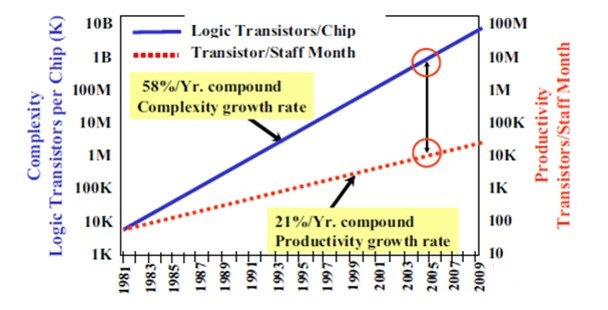
\includegraphics[width=\linewidth]{figures/sematech.jpg}
  \caption{The Productivity Gap
  \cite{industry1999international}}
  \label{fig:sematech}
\end{figure}
Heterogeneous system architectures exploit multiple processor types, to realize the best of both data-parallel and task-parallel (sequential) applications \cite{amd_resources}. To realize the full potential of such systems, the system designers should scrupulously integrate the diverse compute elements available in the platform and allow them to work together seamlessly. While conventional accelerators limit productivity by demanding high skills in hardware engineering, heterogeneous architectures having GPPs and specialized co-processors offer software-like programmability, enhanced application portability and consequently, improved productivity. Some of the popular heterogeneous computing platforms include network processors such as Intel IXP, Embedded systems such as TI OMAP, NVIDIA Tegra and Apple A9, Reconfigurable devices such as Xilinx FPGAs (Virtex, Kintex, etc.) in Zynq platform containing dual core ARM Cortex A9 Processors, General purpose processors such as IBM Cell and ARM big.LITTLE CPU architectures \cite{wiki_nanoscale}. \newline \newline 
These devices guarantee a power-aware design with increased data parallelism and throughput. However, we should also be mindful of the challenges they pose such as different instruction set architectures for different compute elements, varying cache structure and coherence protocols, varying memory access patterns (uniform or non-uniform) and interface types \cite{wiki_nanoscale}, etc. Opaque programming paradigms (like POSIX standard for threads), the differences in underlying micro-architecture and abstractions associated with high-level language programming can impede performance predictions and sometimes, increase power consumption. Designers should explicitly handle thread synchronization and shared variable protection in multi-threaded applications and partition the application suitably between various computing elements. Example: Running a sequential task on FPGA leads to under-utilization of resources and slows down the performance. Similarly, performing SIMD operations on a CPU would be a bad choice. Design decisions generally involve domain expertise and design space exploration, which is a quantitative approach to recognizing the design variables with the most beneficial effect on the system’s performance goals. \newline \newline
To mitigate the challenges listed above, we need to establish a standard programming model that is portable across devices and capable of delivering the desired performance. 
For simple applications, design decisions are straightforward. This prompts us to explore some complex, compute-intensive applications and study the impact of various design decisions on their performance. 
This report deals with the study of two such compute-intensive applications, namely MNIST Digit classifier using Convolutional Neural Network (CNN), and Fully Homomorphic Encryption (FHE), their efficient partitioning between hardware and software and gauging of various design points to achieve a specific optimization goal, i.e. low latency. For example, the first convolutional layer of the MNIST-CNN having a computation demand of 300K multiply-accumulate operations can be processed at 24M MACs/s with single-threaded flow on Intel Core i3 platform, whereas the same platform can process upto 2B MACs/s with multi-threaded OpenCL execution. To achieve sub-microsecond latency, 20 convolution engines (running at 600 MHz) can be used where each engine is able to produce one pixel by performing 25 MAC operations every clock cycle. The peak performance of such a hypothetical engine is 300 billion MAC/sec. In a broader sense, a mere 14 frames/s with sequential flow can be boosted to about 826 frames/s on the same CPU while a cross-platform performance of as high as 3105 frames/s can be accomplished with parallel thread executions. We also present similar analysis for second application (FHE). Here, we focus mainly on the algorithmic design exploration for a specific architecture using high-level synthesis tools.


\section{Contribution}
\label{sect1_2}
The primary focus areas of this thesis can be summarized as follows:
\begin{itemize}
\item Identification and understanding of two applications with high computational complexity which show potential for hardware acceleration.
\item Understanding of programming models best suited for the parallelization of the identified complex applications.
\item Profiling various parts of the applications to isolate the critical paths that need improvement.
\item Performing architectural exploration and suitably partitioning the application between various compute elements available in the platform.
%\item Running and profiling the applications to study the performance improvements with the modified design.
\end{itemize}

\section{Organization}
\label{sect1_3}
The report consists of the following chapters: 
\textbf{Chapter \ref{ch2_background}} presents background knowledge, software and hardware requirements needed for this thesis. 
\textbf{Chapter \ref{ch3_cnn}} delves into the C++ and OpenCL implementation of MNIST Digit Recognition program and studies the runtime benefits with parallel execution.
\textbf{Chapter \ref{ch4_fhew}} explains another complex encryption algorithm implemented in software that exhibits potential for hardware acceleration.
\textbf{Chapter \ref{ch5_conclusion}} draws conclusion to the contents perused in this thesis and throws light on potential direction for future research.
\chapter{Background}
\label{ch2_background}
\section{What is Hardware Acceleration?}
\label{sect2_1}
Migration of some applications originally implemented in software running on a general purpose CPU, to custom hardware acceleration engines, to resolve inherent bottlenecks of the system and improve system performance is referred to as hardware acceleration \cite{wiki_hwacc}. Such specialized accelerators intend to improve portions of the code that incur significant performance overheads such as:
\begin{itemize}
\item Mathematically rigorous functions with more data dependence and reduced control dependence among operations,
\item Repeated routines on different data sets,
\item Other parallelizable tasks, etc. 
\end{itemize}
Some common real-world scenarios demanding the computation bandwidth of hardware accelerators are Audio codec applications, high-speed Video Streaming, Network protocols, Cryptanalysis, Data mining, Natural Language Processing, Computer Vision, etc. \cite{ibm_devworks} The goal is to accomplish a faster execution time in hardware than in software. The hardware execution time includes the actual computation time by the accelerator as well as the communication overheads associated with reading and writing back the data. 

\section{Heterogeneous Platforms}
\label{sect2_2}
Heterogeneous computing platform constitutes different kinds of processors on the same silicon die. Commonly found constituents of an embedded system platform are a general-purpose processor (CPU) and a few specialized co-processors designed for a specific purpose. Examples of co-processors are Digital Signal Processors, which provide Instruction Level parallelism with VLIW, SIMD and superscalar capabilities, GPGPUs and FPGAs. The heterogeneous devices that were used for this project are listed below:
\subsection{Intel Platform with CPU and GPU}
This heterogeneous platform has been chosen to demonstrate code portability across different compute elements, evaluate the runtime of an application in CPU and GPU, analyze whether the given application is control-bound or compute-bound, and estimate the percentage improvement in latency. The \textbf{Intel SDK for OpenCL}\cite{intel_openclSDK} is available for both Windows and Linux Operating Systems and offers packages to run applications on Intel CPU and Graphics Processing Unit. Also, the \textbf{OpenCL Runtime Environment} (RTE) \cite{intel_runtime} provides drivers and library packages required to test applications while they are running. The installation of these packages is easy and will be discussed in detail in Section<TBD>. The CPU used for this thesis is <>(<>cores) running at a clock frequency of <> and the GPU is <> (<> cores) running at a frequency of <>.  
\subsection{Avnet Zedboard with Xilinx Zynq 7000 All-programmable SoC}
This platform comprises of a Processing System with dual-core ARM Cortex A9, running at 667 MHz with NEON SIMD engine and Floating Point Unit, and a Programmable Logic with Artix-7 FPGA. The processing system and programmable logic are connected via AXI Interface. Zedboard has found its place in different market segments, be it Automotive, Consumer Electronics, software-defined Radio applications \cite{dobson2014architecture}, Aerospace and Defense, Medical diagnostics and Imaging, Wired and Wireless communication, Control and Bridging applications \cite{xil_zynqbrief}. Owing to its versatility, this platform has been chosen to conduct experiments on the complex applications at hand.
\section{Programming Models for Hardware Acceleration}
\label{2_3}
The various programming models that have been explored in this thesis are discussed below. The models have been chosen with the view to reducing the burden on the engineers to learn coding at lower levels of abstraction while also achieving unparalleled performance.
\subsection{GPGPUs}
\label{2_3_1}
The first half of this thesis delves into the use of GPGPUs for applications other than their conventional role in computer graphics. The most commonly used programming languages for GPU programming are Open Computing Language (OpenCL) and CUDA. It is interesting to note that CUDA implementations currently support only one vendor, NVIDIA Corporation while OpenCL supports the vendors AMD, Intel, Altera, NVIDIA and Apple.\newline \newline
While OpenCL is open-source, CUDA is proprietary. After a basic run-through of the features of both frameworks such as code portability and flexibility, OpenCL programming model was chosen to carry out the acceleration experiments. The prime focus of this thesis is on OpenCL C APIs, which are maintained by the Khronos group \cite{khronos2008opencl}. The OpenCL architecture is composed of a Host which dispatches commands to the devices. The host CPU offsets loads to the devices and the devices execute these workloads for the host.

\begin{figure}[h!]
  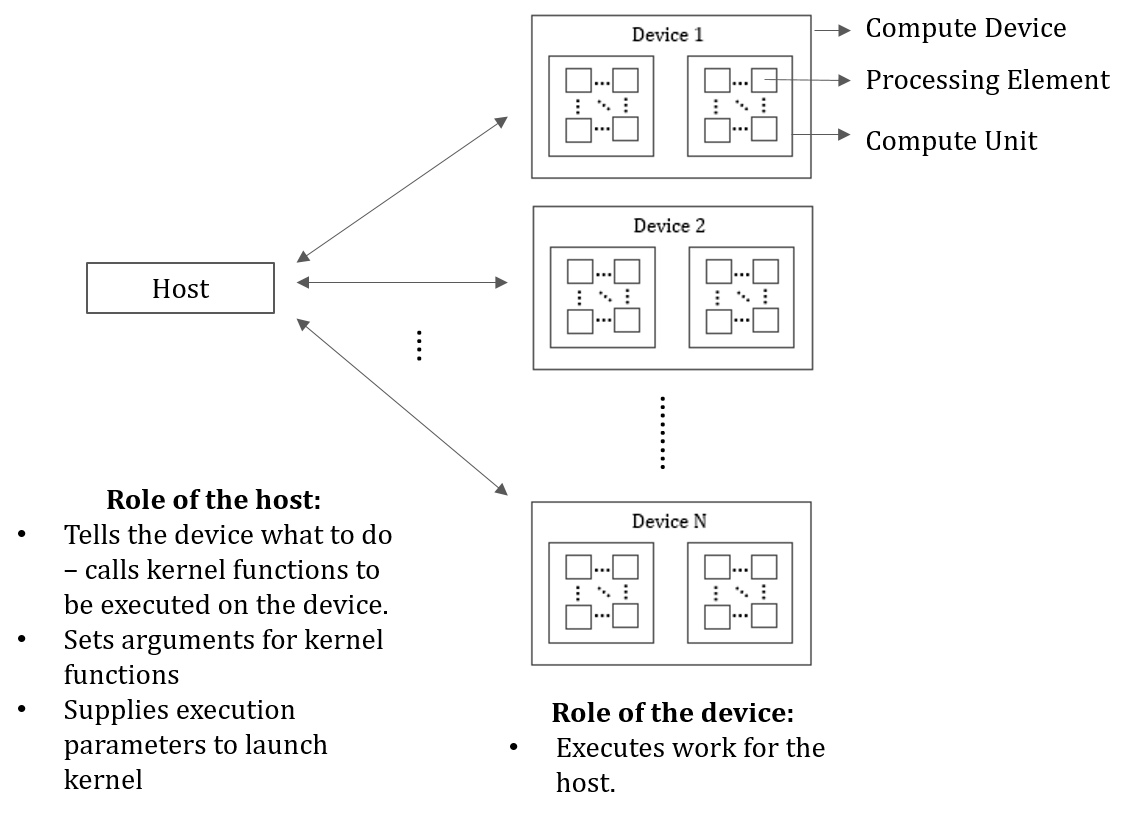
\includegraphics[width=\linewidth]{figures/openCL_architcture.png}
  \caption{The OpenCL Platform Model
  \cite{rosenberg2011opencl}}
  \label{fig:openCL_architecture}
\end{figure}

There are three popular OpenCL Models \cite{opencl_ajg}, which shall be discussed briefly to aid the understanding of internals in OpenCL Programming. 
\subsubsection{Device Model}
\label{2_3_1_1}
It is an abstract view of various components in a Compute device. 
Each device consists of various Compute Units, and each of those compute units are composed of several Processing Elements (PEs). 
Hence, Compute units can be viewed as containers of very simple processors (PEs). 

\begin{figure}[h!]
  \centering
  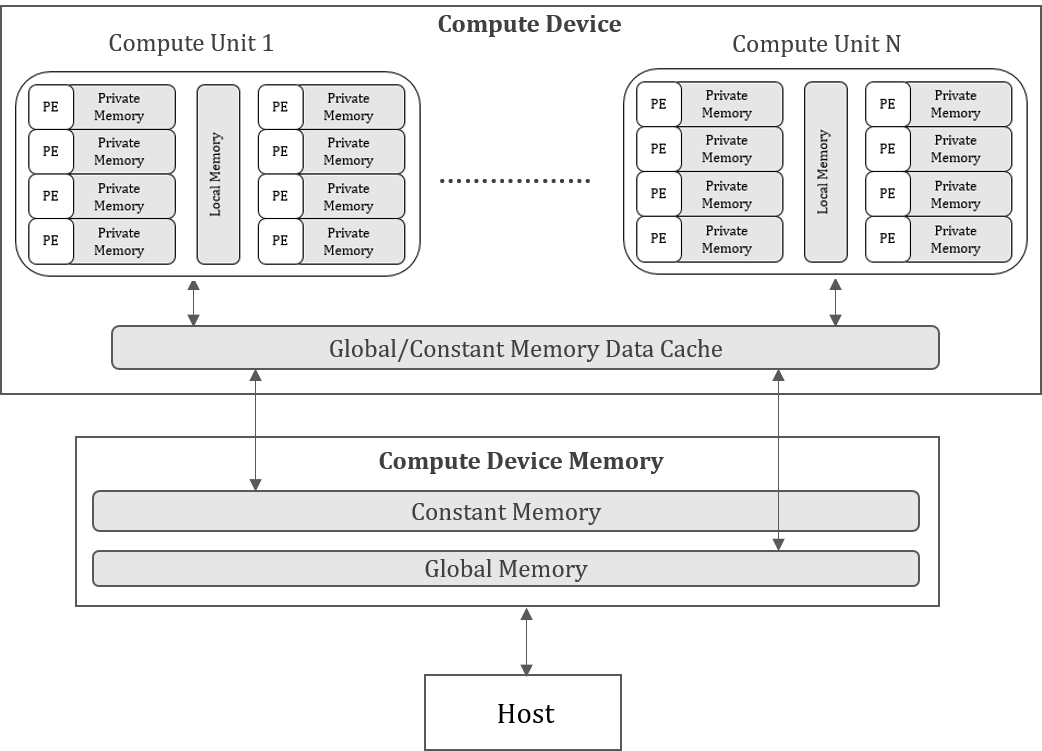
\includegraphics[width=0.80\linewidth]{figures/openCL_deviceModel.png}
  \caption{The Device Model of OpenCL
  \cite{opencl_ajg}}
  \label{fig:openCL_deviceModel}
\end{figure}

\subsubsection{Memory Model}
\label{2_3_1_2}
It defines the memory hierarchy inside an OpenCL device. 
\begin{itemize}
\item \textbf{Global Memory:} Persistent storage accessible by all Processing Elements (PEs) and the host.
\item \textbf{Constant Memory:} Non-persistent, Read-Only Memory shared among all Processing Elements.
\item \textbf{Local Memory:} Shared by all PEs in one Compute Unit and not available to PEs from other compute units. Each Compute Unit has its own local memory.
\item \textbf{Private Memory:} Non-persistent memory accessible by a single Processing Element.
\end{itemize}
\subsubsection{Execution Model}
\label{2_3_1_3}
OpenCL \textbf{kernels} are ordinary functions with special signatures written in OpenCL C, which run on each Processing Element. For data-parallel applications where the same function is invoked several times, the kernels execute in parallel on different PEs over a pre-defined N-dimensional index space \cite{tompson2012introduction}. \newline \newline
A \textbf{work item} is an independent element of execution. It can also be interpreted as the invocation of the kernel for a specific index “i”. The \textbf{global work size} defines the number of work items per work dimension (dimension of the index space).\newline \newline
The host describes an N-dimensional computational load where each index point is represented by a work item. The work items are grouped into \textbf{work groups} by the host and each of these work groups execute in parallel within the compute unit. The work group size is device-dependent and can be found by querying the device using OpenCL APIs. 
Each Compute Unit has its own work-group(s) and each work item in the work group is executed by a single processing element.

\begin{figure}[h!]
  \centering
  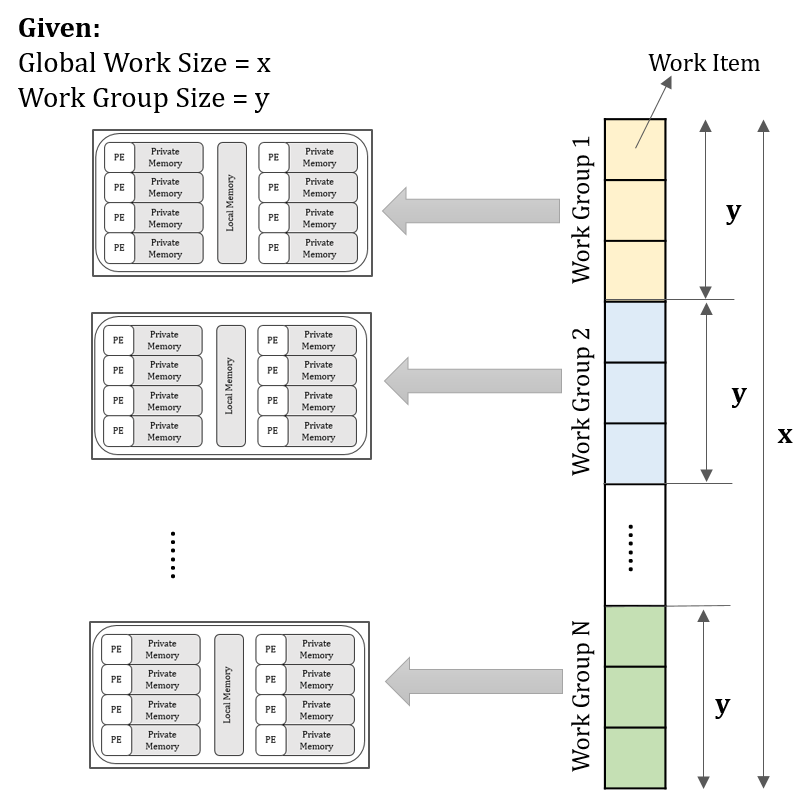
\includegraphics[width=0.70\linewidth]{figures/openCL_workSchedule.png}
  \caption{An Illustration of Data-parallel execution
  \cite{opencl_ajg}}
  \label{fig:openCL_workSchedule}
\end{figure}

\subsection{Field Programmable Gate Arrays}
\label{2_3_2}
\subsubsection{High-Level Synthesis}
\label{2_3_2_1}
Until recently, we were directing our attention to programming in specialized processors using high-level languages such as C and C++. With growing computational demand, a sudden shift in focus to FPGAs necessitated the hardware programming knowledge among software engineers. \newline \newline
The Figure \ref{fig:graph-rtldesign} depicts implementation time for various programming models and we notice that RTL design, although the most beneficial in terms of performance compared to standard and specialized processors, demands the highest development time, beyond the acceptable software development time, to capture the market. This can be attributed to the increased concretization in the design at lower-levels and the deficit of hardware programming experience and expertise.
\begin{figure}[h!]
  \centering
  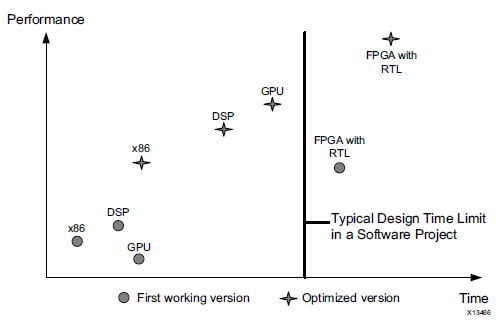
\includegraphics[width=0.8\linewidth]{figures/graph-rtldesign.png}
  \caption{Performance vs. Design Time with RTL Design
  \cite{xil_hls}}
  \label{fig:graph-rtldesign}
\end{figure}
To relieve the engineers of this burden and improve the time-to-market, High-Level Synthesis tools which eliminate the differences in programming models of processors and FPGAs have been introduced. HLS tools translate a C/C++ specification into an equivalent RTL description. The Figure \ref{fig:graph-hlsdesign} illustrates the performance peaks that can be accomplished with High-Level Synthesis, in comparison to standard processors and GPUs. 
\begin{figure}[h!]
  \centering
  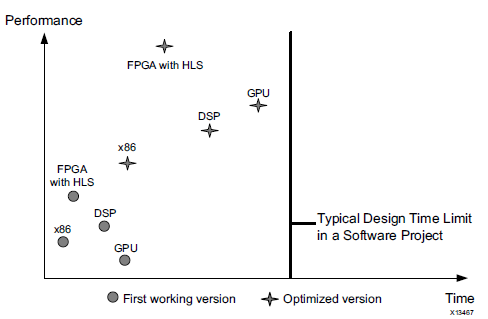
\includegraphics[width=0.8\linewidth]{figures/graph-hlsdesign.png}
  \caption{Performance vs. Design Time with HLS Compiler
  \cite{xil_hls}}
  \label{fig:graph-hlsdesign}
\end{figure}
It is only fair that we acknowledge the fact that RTL code automatically generated by HLS tools may not be the most optimal implementation. It may not fully exploit the parallelism offered by the underlying hardware, unlike the design with HDL languages. However, it meets the time limit specified for software development in many cases and hence proves very useful in that respect.\newline \newline 
Pointers are supported in HLS when they can be completely described at compile-time, without any need for runtime intelligence. FPGA-based designs using HLS demand the data and size of memory blocks to be deterministic at compile-time. This static memory allocation facilitates realization of an algorithm’s memory as a register, FIFO or Block RAM \cite{xil_hls}. \newline \newline
Register-based memory implementation is the fastest as a register is an independent entity, which doesn’t require any addressing logic. FIFOs are used to transfer data between loops and functions. It is a queue with a single entry and exit point. FPGAs have dedicated Random-access memory blocks called Block RAMs which retain values for as long as the system is powered on. Block RAMs support parallel access of two different memory locations. \newline \newline
HLS tools provide easy testing of functional correctness in both C and RTL implementations and offer numerous optimization directives, which when aptly used, help accomplish several performance goals. 
\subsubsection{OpenCL}
\label{2_3_2_2}
OpenCL standard facilitates implementing parallel algorithms at higher levels of abstraction on FPGAs as opposed to traditional low-level programming using Hardware Description Languages such as VHDL and Verilog \cite{opencl_vhblog}. The drawbacks of High-level Synthesis tools in this respect is that they take in a sequential C description and try to extract thread-level parallelism out of it. Failure to gain the maximum parallelism beats the purpose of using an FPGA. Thus, OpenCL standard allows spawning of threads and annotating them with explicit constructs that describe parallelism and memory access hierarchy (execution parameters discussed in Figure \ref{fig:openCL_architecture}).\newline \newline
Unlike the CPU-GPU platform where concurrent threads are run on different cores, kernels are translated to equivalent dedicated circuits which implement each function in the hardware. These circuits are wired appropriately to simulate the dataflow in the kernel \cite{singh2011implementing}. The final circuit implemented on FPGAs is heavily pipelined and exhibits multi-threading capabilities, offering a final design with pipelined parallelism.\newline \newline
In conventional RTL design, the designers should handle cycle-wise hardware descriptions, create data paths, create FSMs for control flow, manage timing constraints and integrate low-level IP cores to the design, all by themselves. OpenCL Compiler automates these steps and helps shift the focus to refining the algorithm rather that detailing the hardware design. OpenCL being a cross-platform standard can be easily carried forward to different FPGA generations with little design effort, while the benefits of improved capabilities and performance remain intact \cite{singh2011implementing}.
\begin{figure}[h!]
  \centering
  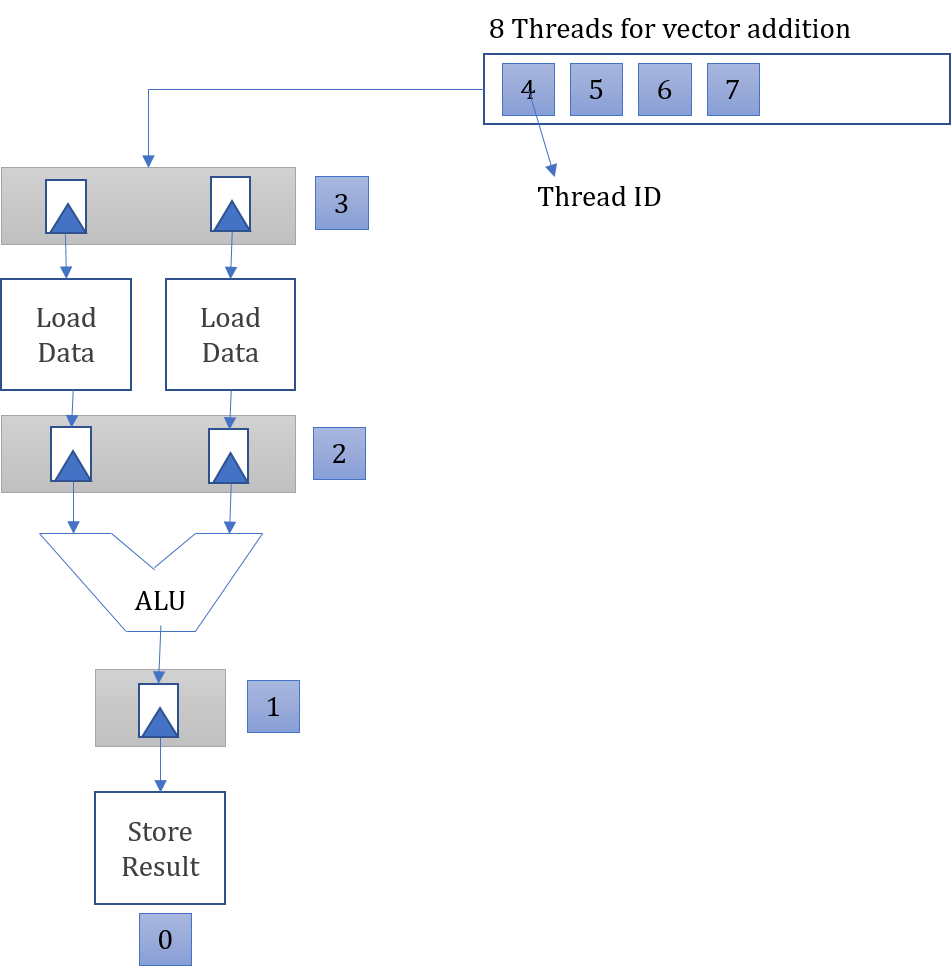
\includegraphics[width=0.6\linewidth]{figures/pipelined_parallelism_fpga_opencl.png}
  \caption{Pipeline Parallelism achieved by OpenCL-to-FPGA compiler
  \cite{singh2011implementing}}
  \label{fig:pipeline_parallelism_fpga_opencl}
\end{figure}
Figure \ref{fig:pipeline_parallelism_fpga_opencl} depicts the pipelined execution of the 8 threads by the generated circuit. Assuming there are three pipeline stages, at cycle 3, we observe that thread 0 stores the computed result, thread 1 computes the sum for a new set of data values, thread 2 copies the values read from memory while thread 3 reads data from the memory. Thus, at any point during the execution, all pipeline stages manipulate a different thread and all stages of the pipeline are active, until the processing of all threads are complete. \newline \newline
Some FPGA vendors like Xilinx and Altera offer OpenCL SDKs for FPGAs. We are not using the Altera Toolchain for our experiments, but the benchmark code taken for test relies on some platform-independent C++ headers and includes that are available with this SDK (Example: aocl\_utils.h). Hence, this thesis shall make use of Altera OpenCL (AOCL) SDK to analyze and modify the code and study the results.

\chapter{Hardware Acceleration using Graphics Processing Unit}
\label{ch3_cnn}
Deep Learning is an avant-garde approach to imparting knowledge to the machines to achieve the ultimate goal of artificial intelligence without explicit coding, and bridge the current gap between technology integration and expertise. It is of interest in several domains\cite{wiki_ml}, such as:
\begin{itemize}
\item Self-driving cars, Automated flight control, Handwriting and Voice recognition software, which are real-time and cannot be programmed by hand or require intense effort doing so manually.
\item Database Mining.
\item Applications with Product Recommendations in e-commerce websites such as Amazon and Netflix, which are essentially self-customizing.
\item Understanding of the human genome.
\item Anti-Spam filters and Intelligent Search bars in browsers.
\end{itemize} 
Claims have been made that off-the-shelf accelerators in the embedded platforms offer an edge over CPU-based systems in deep learning computations\cite{hegde2016caffepresso}. We seek to validate the efficiency of deep-learning methods on heterogeneous architectures with a simple Lenet-5 Model of MNIST Dataset classifier. 
\section{Deep Learning using Convolutional Neural Networks}
\label{3_1}
The Figure \ref{fig:ML_Classification} shows the most common types of learning algorithms. The choice of the algorithm depends on the problem we intend to solve.
\begin{figure}[h!]
  \centering
  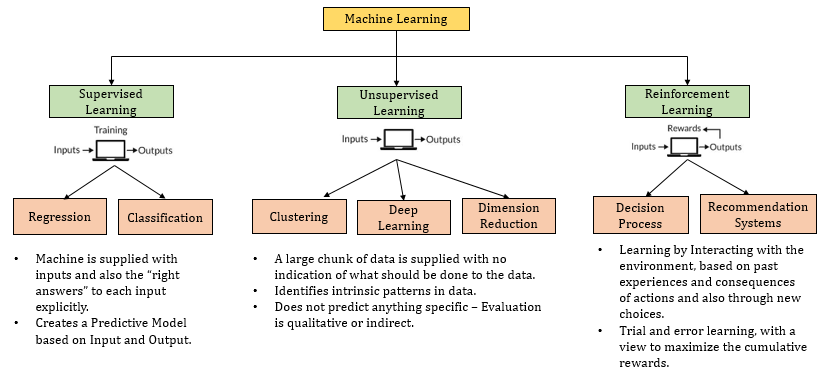
\includegraphics[width=\linewidth]{figures/ML_Classification.PNG}
  \caption{Types of Machine Learning Algorithms
  \cite{upx_ml}}
  \label{fig:ML_Classification}
\end{figure}
\newline Various experiments have substantiated the claim that Convolutional Neural Networks (also called ConvNets or CNNs) outperform other gradient-based learning techniques in handling variable input dimensions in the 2-dimensional space \cite{lecun1998gradient}.
Multilayer ConvNets with back-propagation can be exploited to build a strong decision layer capable of classifying data of high dimensionality, with minimal processing. \newline \newline
Any character recognition system is comprised of the following two parts:\newline
1.	\textbf{Feature Extractor }– \newline
It transforms the input into low-dimensional feature vectors which comprise of only the relevant information of interest from the huge input data \cite{wiki_fe}. The chosen features are essentially invariant to the transformations and distortions that are applied to the input. 
\newline
Feature extraction attempts to reduce the complexity that stems from high input dimensionality, by downsizing the data while still accomplishing reasonable accuracy in the description of data \cite{wiki_fe}. Feature extractors are application-specific.\newline \newline
2.	\textbf{Classifier} – \newline
It is a trainable general-purpose entity which analyzes the data and categorizes the feature vectors appropriately into classes. The accuracy of a classifier is predominantly decided by the features selected in the feature extraction process. \newline
The efficiency of a classifier is determined not just by the correctness in categorizing a given set of test input samples but also the error rate. 
\begin{figure}[h!]
  \centering
  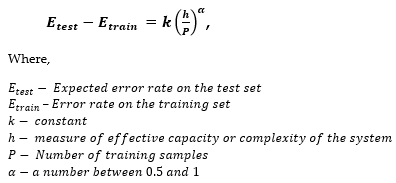
\includegraphics[width=0.7\linewidth]{figures/classifier_efficiency_formula.PNG}
  \caption{Formula to determine Classifier Efficiency
  \cite{lecun1998gradient}}
  \label{fig:classifier_efficiency_formula}
\end{figure}
\newline Studies have revealed the relationship between expected error rate on test set and error rate on training set as shown in Figure \ref{fig:classifier_efficiency_formula}. The difference between these two error values decreases as the number of training samples increases. Also, if the complexity of the system “h” increases, training error decreases. Hence, we infer that the system becomes more robust with more training. 
\newline \newline
The traditional machine learning approach involves handcrafting features of interest, which can take painstaking amount of time and effort, coupled with domain expertise. Feature engineering in Deep nets is automatic and more accurate in comparison to conventional methods \cite{dlintro_am}.
\begin{figure}[h!]
  \centering
  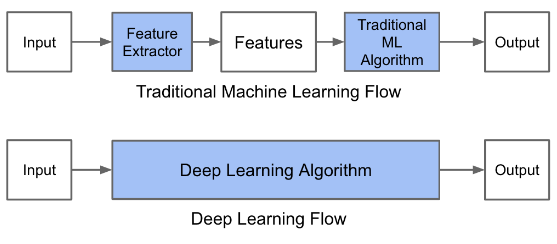
\includegraphics[width=0.7\linewidth]{figures/dlvsml.png}
  \caption{Learning differences - Traditional vs. Deep Learning
  \cite{dlintro_am}}
  \label{fig:deep_learning_flow}
\end{figure}
\newline
Owing to high computational complexity, CNN usage is restricted, especially in portable devices \cite{gysel2016hardware}. 

\subsection{MNIST Digit Recognition using Lenet-5 ConvNet}
\label{3_1_1}
The Lenet-5 Architecture for handwritten digit recognition was first conceived by LeCun et al. in 1998. The MNIST(Modified National Institute of Standards and Technology) database consisting of 60000 training samples and 10000 test inputs available for download in \cite{mnist_database} was used for the experiments discussed in the paper \cite{lecun1998gradient}. This paper proved the general consensus \ref{fig:deep_learning_flow}  that ConvNets eliminate the need for hand-made feature extractors and are the most efficient. Today, Artificial Intelligence is a buzzword and almost all AI related applications are leveraging ConvNets to achieve the best performance with low runtime complexities. 
\begin{figure}[h!]
  \centering
  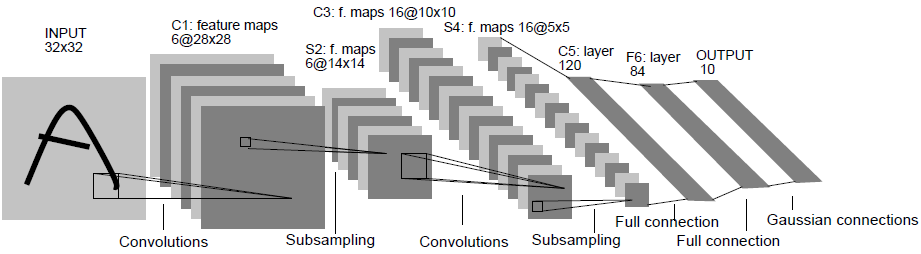
\includegraphics[width=\linewidth]{figures/Lenet-5-org.PNG}
  \caption{Original Lenet-5 ConvNet Architecture; Each plane represents a feature map in which weights are shared.
  \cite{lecun1998gradient}}
  \label{fig:Lenet-5-org}
\end{figure}
Figure \ref{fig:Lenet-5-org} shows the original Lenet-5 architecture described in \cite{lecun1998gradient}. 
It is important to understand the purpose of various layers of the Lenet-5 ConvNet architecture to study their runtime in the application. The following subsections shall describe the layers in detail.
\subsubsection{Convolution Layer \cite{cnn_ak}}  
\begin{figure}[h!]
  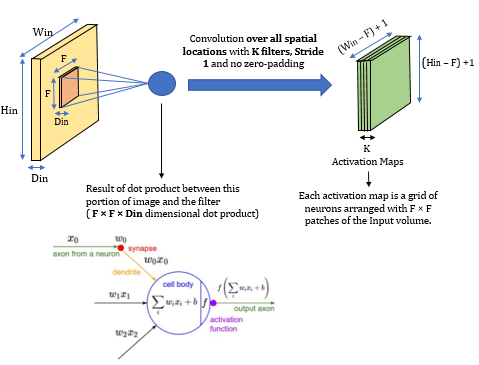
\includegraphics[width=\linewidth]{figures/ConvLayer.PNG}
  \caption{Convolution Layer
  \cite{cnn_ytak}}
  \label{fig:ConvLayer}
\end{figure}
Convolution Layer is the core of a ConvNet. Consider an input volume of height $H_i$, width $W_i$ and depth $D_i$. The depth indicates the color channels, i.e. the third dimension of input volume which can be activated. A filter of dimension F × F is slid over the input image spatially to evaluate dot products between the input image volume and the filter, thus generating 2-dimensional activation maps. The filter spans through the depth of the input image. 
\newline \newline Activation map is a visualization of which portions of the input volume are responding to the filter. For example, if the filter is intended to filter out vertical lines, activation map is representative of filter activations on the image. i.e. it contains all portions of the image which are likely to have vertical lines.  Usually, several filters, also called kernels are convolved with the input image, resulting in several activation maps stacked in the depth dimension. In a ConvNet, there are several convolution layers and intuitively, they build up an entire feature hierarchy. 
\newline
Each stage builds up very specific features which filters in the subsequent stages will be excited about. i.e. piece by piece, we create 3-D volumes of higher levels of abstraction than the previous stage\cite{zeiler2014visualizing}.\newline \newline
\begin{figure}[h!]
  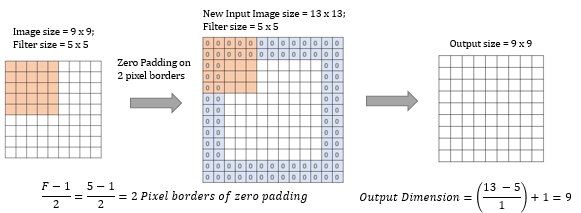
\includegraphics[width=\linewidth]{figures/zero_padding_conv.PNG}
  \caption{Preserving Input dimensions using Zero Padding
  \cite{cnn_ytak}}
  \label{fig:zero_padding_conv}
\end{figure}\underline{\textbf{\emph{\large Generalization of Concepts:}}}\newline
\textbf{Required Hyperparameters:}
	\begin{adjustwidth}{2cm}{}
       Number of filters, K \newline
       Spatial Extent of the filter, F \newline
       Stride, S \newline
       Quantum of Zero padding, P (Figure \ref{fig:zero_padding_conv})
	\end{adjustwidth}
\textbf{Input Dimensions:} $W_1$×$H_1$×$D_1$ \newline
\textbf{Output Dimensions:} $W_2$×$H_2$×$D_2$, 
	\begin{adjustwidth}{2cm}{}
      Where \newline 
	  $D_2$ = K \newline
	  $W_2$ = (($W_1$ – F +2P)/S) + 1 \newline
	  $H_2$ = (($H_1$ – F +2P)/S) + 1 \newline
    \end{adjustwidth}
Each filter has an associated bias. The value 1 is added in the above formulae to account for that bias. Stride is the distance by which the filter is slid around the input volume.\newline
Hence, total number of parameters introduced in the neural network is given by (F . F. $D_1$) × K weights and K biases. For computational convenience, K is usually set as powers of 2. Some libraries branch into special routines when encountering powers of 2, and these routines are highly optimized and efficient for computations in a vectorized form \cite{cnn_ytak}. \newline \newline
The output of a filter covering a particular region of the input x can be interpreted to be a neuron fixed in space, which computes $w^T$x + b. The connections of the neuron are localized and this connectivity expands up to the receptive field of the neuron, given by the filter size F × F. An activation map can be perceived as a grid of neurons with shared weights and representing the dot products of each F × F patch of the input volume. As there can be multiple filters in a single convolution layer, the resultant output is a 3-D volume of neurons, as illustrated in Figure \ref{fig:ConvLayer_1}. This 3-D volume has shared parameters spatially (H×W – within the same depth slice) but across depth, the parameters are different. The neurons illustrated in the Figure \ref{fig:ConvLayer_1} are all acting on the same input patch but with different weights. 
\begin{figure}[h!]
  \centering
  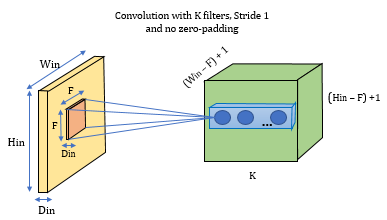
\includegraphics[width=0.7\linewidth]{figures/ConvLayer_1.PNG}
  \caption{3-dimensional volume of Neurons
  \cite{cnn_ytak}}
  \label{fig:ConvLayer_1}
\end{figure}
\subsubsection{MaxPool Layer}
\begin{figure}[h!]
\centering
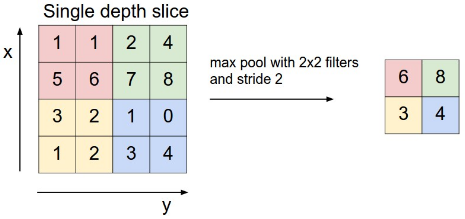
\includegraphics[width=0.7\linewidth]{figures/maxpool.PNG}
\caption{Max Pooling
\cite{cnn_ak}}
\label{fig:maxpool}
\end{figure}
Down-sampling layer which operates independently on all activation maps.
\textbf{Required Hyperparameters:}
  \begin{adjustwidth}{2cm}{}
  Spatial Extent of the filter, F \newline
  Stride, S 
  \end{adjustwidth}
\textbf{Input Dimensions:} $W_1$×$H_1$×$D_1$ \newline
\textbf{Output Dimensions:} $W_2$×$H_2$×$D_2$ 
  \begin{adjustwidth}{2cm}{}
  Where \newline
  $W_2$ = (($W_1$-F)/S)+1 \newline
  $H_2$ = (($H_1$-F)/S)+1 \newline
  $D_2$ = $D_1$
  \end{adjustwidth}
Example of Maxpool operation with filter size 2 × 2 and Stride 2 is illustrated in Figure \ref{fig:maxpool}.
\subsubsection{Inner Product Layer}
\begin{figure}[h!]
  \centering
  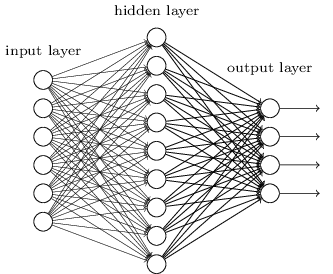
\includegraphics[width=0.5\linewidth]{figures/FCLayer.png}
  \caption{Inner Product Layer
  \cite{cnn_ak}}
  \label{fig:FCLayer}
\end{figure}
It is also called the fully connected layer as the neurons of this layer are pairwise fully connected with the neurons of the previous (input) layer. The neurons within the same layer do not share connections.
\subsubsection{ReLU Layer}
\begin{figure}[h!]
  \centering
  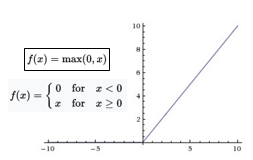
\includegraphics[width=0.5\linewidth]{figures/relu.PNG}
  \caption{ReLU Function in Neural Networks
  \cite{wiki_relu}}
  \label{fig:relu}
\end{figure}
Rectified Linear Unit \cite{nair2010rectified} is a non-linear activation function described by Figure \ref{fig:relu}, commonly used in neural networks for the purpose of thresholding after convolution. ReLU is faster compared to other activation functions such as sigmoid and tanh units as it does not involve any normalization or exponential calculation, unlike its counterparts. 
\subsubsection{Softmax Layer}
\begin{figure}[h!]
  \centering
  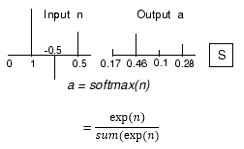
\includegraphics[width=0.3\linewidth]{figures/softmax.PNG}
  \caption{Softmax Function
  \cite{mathworks_softmax}}
  \label{fig:softmax}
\end{figure}
MNIST Digit Classifier has ten class labels for the ten digits 0 to 9, which are mutually exclusive. An ideal classifier should assign a probability of 1 to one of the ten possible nodes at the output and assign 0 probability to others. Due to difficulty in realizing this, we use Softmax function usually in the last layer of the ConvNet, which increases the probability of the maximum value from the previous stage in such a way that sum of the output probabilities of the 10 classes is 1 \cite{softmax_cmc}.
\subsubsection{Modified Hyperparameters for MNIST Dataset}
\begin{figure}[h!]
  \centering
  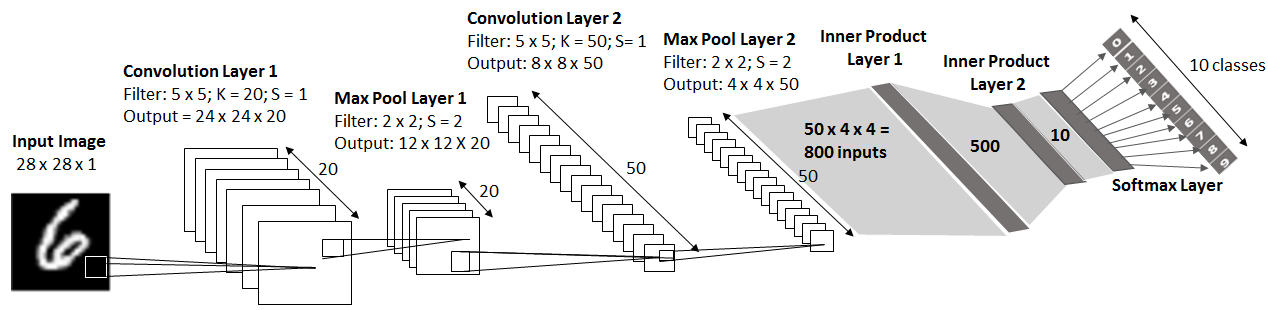
\includegraphics[width=\linewidth]{figures/Lenet-5-papaa.PNG}
  \caption{Lenet-5 CNN Architecture for MNIST Dataset with modified hyperparameters
  \cite{papaa-opencl}}
  \label{fig:Lenet-5-MNIST}
\end{figure}
Different versions of MNIST Datasets have been introduced over the years. The first version had images centred within the 28×28 region and it was extended to 32×32 images by adding extra background pixels \cite{lecun1998gradient}. In the later versions of the database, images were normalized in size to fit a 20×20 field, forming the centre of mass of the resultant 28×28 image. The Architecture illustrated in the Figure \ref{fig:Lenet-5-org} uses 32×32 images while the benchmark code \cite{papaa-opencl} that will be used for our experiments uses 28x28 images. Table \ref{table:hyperparams} defines the hyper-parameters for the different layers of the MNIST/Lenet-5 CNN benchmark application\cite{papaa-opencl}.
\begin{table}
\begin{tabular}
{|m{6em}|m{6em}|c|c|}
\hline
\centering \textbf{Layers} & \textbf{\makecell{Input\\Dimensions}} & \textbf{\makecell{Hyper-\\parameters}} & \textbf{Output Dimensions}\\
\hline
\centering Convolution Layer 1 & \makecell[l]{$W_1$×$H_1$×$D_1$=\\28×28×1} & \makecell[l]{F = 5,\quad S = 1,\\K = 20,\quad P = 0} & \makecell[l]{$W_2$ = ((28-5)/1)+1 = 24\\$H_2$ = ((28-5)/1)+1 = 24\\$W_2$ = 20}\\
\hline
\centering MaxPool Layer 1 &\makecell[l]{$W_1$×$H_1$×$D_1$=\\24×24×20}&\makecell[l]{F = 2,\quad S = 2}&\makecell[l]{$W_2$ = ((24-2)/2)+1 = 12\\$H_2$ = ((24-2)/2)+1 = 12\\$W_2$ = 20}\\
\hline
\centering Convolution Layer 2 & \makecell[l]{$W_1$×$H_1$×$D_1$=\\12×12×20} & \makecell[l]{F = 5,\quad S = 1,\\K = 50,\quad P = 0} & \makecell[l]{$W_2$ = ((12-5)/1)+1 = 8\\$H_2$ = ((12-5)/1)+1 = 8\\$W_2$ = 50}\\
\hline
\centering MaxPool Layer 2 &\makecell[l]{$W_1$×$H_1$×$D_1$=\\8×8×50}&\makecell[l]{F = 2,\quad S = 2}&\makecell[l]{$W_2$ = ((8-2)/2)+1 = 4\\$H_2$ = ((8-2)/2)+1 = 4\\$W_2$ = 50}\\
\hline
\centering Inner Product Layer 1 &\makecell[l]{(4×4×50=800)\\ \\$W_1$×$H_1$×$D_1$=\\1×1×800 \\(Vector of\\matrices)}&\makecell[l]{Number of Outputs\\= 500 (defined in\\ lenet5Model.h)} &\makecell[c]{500\\ (Vector of float values)}\\
\hline
\centering ReLU\\Layer &\centering 500& - &500\\
\hline
\centering Inner Product Layer 2 &\centering 500& \makecell[l]{Number of Outputs\\= 10 (defined in\\ lenet5Model.h)} &10\\
\hline
\centering Softmax Layer &\centering 10& - &10\\
\hline
\end{tabular}
\caption{Hyperparameters for Lenet-5 CNN described in MNIST/Lenet-5 ConvNet Benchmark code\cite{papaa-opencl}}
\label{table:hyperparams}
\end{table}
\subsection{Experiments with C++ Code}
\label{3_1_2}

\subsubsection{Prerequisites}
\label{3_1_2_1}
Performance Application Programming Interface (also called PAPI) offers interfaces to hardware performance counters in the underlying platform. These counters count the number of occurrences of a specific event or signal related to the functioning of the processor. This library is used to benchmark the test application and can be installed as follows:
\begin{scriptsize}
\linuxbash
\begin{lstlisting}
$ sudo apt-get install papi-tools
\end{lstlisting}
\end{scriptsize}
Download PAPI files from the official PAPI Website \cite{papi_official}.
\begin{scriptsize}
\linuxbash
\begin{lstlisting}
$ wget http://icl.cs.utk.edu/projects/papi/downloads/papi-5.5.0.tar.gz
\end{lstlisting}
\end{scriptsize}
Extract the tar file and open the directory:
\begin{scriptsize}
\linuxbash
\begin{lstlisting}
$ tar -zxvf papi-5.5.0.tar.gz
$ cd papi-5.5.0
\end{lstlisting}
\end{scriptsize}
Follow the steps specified in the file INSTALL.txt inside the PAPI directory.\newline
As the Makefile is not already available, we create the Makefile using the command:
\begin{scriptsize}
\linuxbash
\begin{lstlisting}
$ sudo ./configure
\end{lstlisting}
\end{scriptsize}
After the creation of Makefile, compile and link the library using the command (spawn as many parallel threads as is supported by the number of CPUs in the system):
\begin{scriptsize}
\linuxbash
\begin{lstlisting}
$ sudo make -j24
\end{lstlisting}
\end{scriptsize}
To check for errors, perform a simple test:
\begin{scriptsize}
\linuxbash
\begin{lstlisting}
$ sudo make test -j24
\end{lstlisting}
\end{scriptsize}
To run all the available test programs:
\begin{scriptsize}
\linuxbash
\begin{lstlisting}
$ sudo make fulltest -j24
\end{lstlisting}
\end{scriptsize}
Navigate to the directory when the benchmark code using PAPI is located and link the code to PAPI library by setting the following environment variable:
\begin{scriptsize}
\linuxbash
\begin{lstlisting}
$ export LD_LIBRARY_PATH=/usr/local/lib
\end{lstlisting}
\end{scriptsize}
\subsubsection{Existing Code Flow Description}
\label{3_1_2_2}
Figure \ref{fig:CPP_flow_lenet5} shows the code flow in software. The model is pre-trained using Caffe framework and the weights and biases are stored in the file lenet5\_model.cpp for use in the main application.\newline
There are two Application modes, namely \textit{Sample} and \textit{Test}. The \textit{Sample} mode is used when a MNIST single image has to be identified. The \textit{Test} mode is to test the full MNIST dataset, compare the predicted digit against the pre-defined image label and calculate the prediction accuracy.\newline\newline
\begin{figure}[h!]
\centering
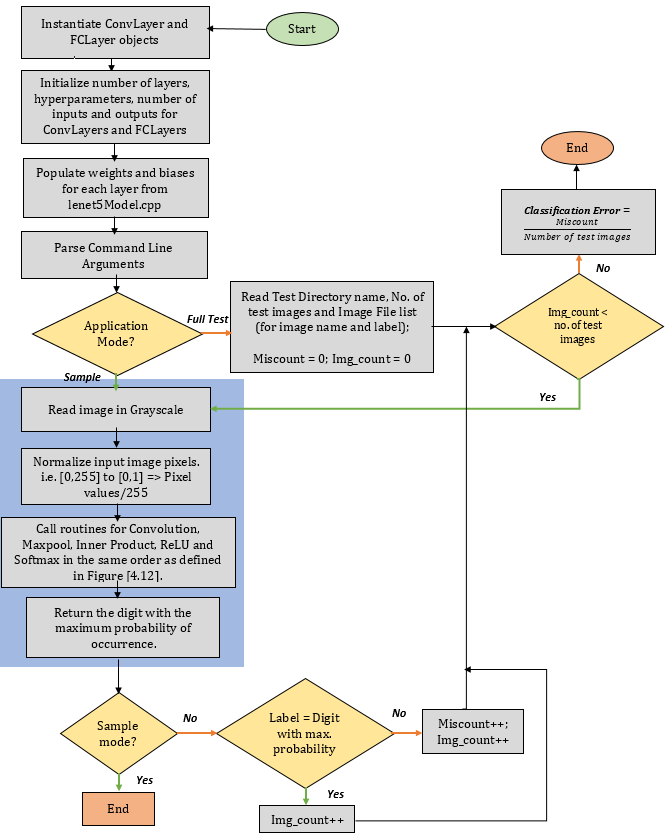
\includegraphics[width=\linewidth]{figures/CPP_flow_lenet5.png}
\caption{Software Code Flow
\cite{papaa-opencl}}
\label{fig:CPP_flow_lenet5}
\end{figure}\textbf{Compilation Steps \cite{papaa-opencl}} \newline\newline
\underline{To compile the code:}
\begin{scriptsize}
\linuxbash
\begin{lstlisting}
$ make all
\end{lstlisting}
\end{scriptsize}
\underline{To test a sample image:}
\begin{scriptsize}
\linuxbash
\begin{lstlisting}
$ ./lenet_app -m sample -i <image_path>
\end{lstlisting}
\end{scriptsize}
Example: 
\begin{scriptsize}
\linuxbash
\begin{lstlisting}
$ ./lenet_app -m sample -i ../imgs/mnist_test_img_0.pgm
\end{lstlisting}
\end{scriptsize}
\underline{To test the full MNIST Dataset:}
\begin{scriptsize}
\linuxbash
\begin{lstlisting}
$ ./lenet_app -m test -f <image_list_file> -d <image_dir> [-n <no_images_to_test>]
\end{lstlisting}
\end{scriptsize}
Example: 
\begin{scriptsize}
\linuxbash
\begin{lstlisting}
$ ./lenet_app -m test -f ../imgs/mnist_test_img_list.csv -d ../imgs/mnist-testset
\end{lstlisting}
\end{scriptsize}
The .csv image list file contains all MNIST handwritten images sized 28x28, along with their labels. These labels help calculate the prediction accuracy and error probability of the digit classifier.\newline
\textbf{Acceleration Hot-spots} \newline 
In order to identify the acceleration hot-spots, each operation of the ConvNet was profiled and the results were observed as illustrated in Table \ref{table:sw_hotspots}. The total application runtime (execution of all 8 layers) is around 77269 $\mu$s = 0.077 seconds. The API \textit{\textbf{PAPI\_get\_virt\_usec()}} is used to get the timestamp in microseconds. To use this API, header file "papi.h" has to be included in the source file.
\begin{table}[htbp]
\caption{Analysis of Application Hot-spots for Acceleration}
\centering
\begin{tabular}{l c}
\toprule
\textbf{Layers }& \textbf{Computation Time ($\mu$s)}\\
\midrule
Convolution 1 &12308\\
\midrule
MaxPool 1 &3382\\
\midrule
Convolution 2 &48164\\
\midrule
MaxPool 2 &559\\
\midrule
Inner Product 1 &5522\\
\midrule
ReLU&12\\
\midrule
Inner Product 2 &73\\
\midrule
Softmax&9\\
\bottomrule
\end{tabular}
\label{table:sw_hotspots}
\end{table}
The convolution layer involves about 86\% ((12308+48164)/70029) of the required arithmetic operations in the ConvNet framework. Following this, the fully connected layers are the next most resource-intensive layers. 
\subsubsection{Improvements}
\label{3_1_2_3}
One approach to minimizing data transfer to off-chip memory is by using reduced bit-width fixed point numbers, realizable by using open-source fixed point arithmetic libraries like LibFi \cite{LibFi}. This approach is very straightforward and promises speedup, reduced area and consequently reduced energy consumption. However, the specifics of this approach are beyond the scope of this thesis. \newline \newline
We intend to port the various layers of the ConvNet into Graphics Processing Unit for concurrent execution and significant speedup. This requires some understanding of the OpenCL device models discussed in Section \ref{2_3_1}
Each platform comes with a ready-to-use library which may pose optimization challenges, especially when designing larger applications.  Yet another challenge is mapping, owing to differences in on-chip memory, kinds of parallelism that a particular accelerator can support and communication bandwidth. We seek to accelerate the layers of the ConvNet by using fine-grained GPUs which exhibit a high degree of data-parallelism.
\subsection{Experiments with OpenCL Code}
\label{3_1_3}
\subsubsection{Pre-requisites}
\label{3_1_3_1}
\subsubsection*{OpenCL Setup in Ubuntu 14.04}
The following are required to run OpenCL Applications on the system: 
\begin{itemize}
\item Drivers to support OpenCL - Already available in current GPUs
\item OpenCL Headers
\item Vendor-specific libraries (specific to Intel, NVIDIA, AMD, etc.)
\item Installable client driver (.icd)
\item libOpenCL.so 
\end{itemize} \textbf{1. Installing OpenCL Headers \cite{opencl_headers}:} \newline
Navigate to the path \textit{/usr/include} and create a directory named CL.
\begin{scriptsize}
\linuxbash
\begin{lstlisting}
$ sudo apt-get install opencl-headers
\end{lstlisting}
\end{scriptsize}
\textbf{2. Installing vendor-specific libraries} \newline
As Intel CPU is used for our experiments, the following packages are to be installed:
\begin{itemize}
\item OpenCL™ Runtime 16.1 for Intel Core™ and Intel Xeon Processors for Ubuntu (64-bit) \cite{intel_runtime}
\item Intel SDK for OpenCL™ Applications \cite{intel_openclSDK}
\end{itemize}
After navigating to the respective installation directories, the command: 
\begin{scriptsize}
\linuxbash
\begin{lstlisting}
$ sudo ./install.sh
\end{lstlisting}
\end{scriptsize}
is used to initiate installation. \newline\newline
\textbf{Dependencies:}\newline \newline
\textbf{mono-devel} package (Installation steps summarized in \cite{mono-devel}).\newline Other missing packages are usually prompted during installation and can be installed using the command: 
\begin{scriptsize}
\linuxbash
\begin{lstlisting}
$ sudo apt-get install <package_name>
\end{lstlisting}
\end{scriptsize}
Extract the SDK tarball and navigate to the extracted directory:
\begin{scriptsize}
\linuxbash
\begin{lstlisting} 
$ tar -xzvf intel_sdk_for_opencl_2016_ubuntu_6.3.0.1904_x64.tgz
$ cd intel_sdk_for_opencl_2016_ubuntu_6.3.0.1904_x64
\end{lstlisting}
\end{scriptsize}
The rpm directory contains many default packages for RedHat Linux with \textbf{.rpm} extension. They need to be converted to \textbf{.deb}(Debian) files to be installed in Ubuntu. To handle .rpm files, \textbf{libnuma} package is required:
\begin{scriptsize}
\linuxbash
\begin{lstlisting} 
$ sudo apt-get install -y rpm alien libnuma1
\end{lstlisting}
\end{scriptsize}
To \textbf{convert rpm format to deb} format and install the Debian packages: 
\begin{scriptsize}
\linuxbash
\begin{lstlisting}        
$ alien *.rpm
$ dpkg -i *.deb 
\end{lstlisting}
\end{scriptsize}
\textbf{3. Installing the Intel OpenCL ICD Loader}
\begin{scriptsize}
\linuxbash
\begin{lstlisting}
$ sudo ln -s /opt/intel/opencl-1.2-5.2.0.10002/etc/intel64.icd /etc/OpenCL/vendors/intel64.icd
\end{lstlisting}
\end{scriptsize}
\textbf{4. Installing a symbolic link to libOpenCL.so} 
\begin{scriptsize}
\linuxbash
\begin{lstlisting}
$ sudo ln -s /opt/intel/opencl-1.2-5.2.0.10002/lib64/libOpenCL.so /usr/lib/libOpenCL.so 
$ sudo ldconfig
\end{lstlisting}
\end{scriptsize}
To check if OpenCL applications run properly, clone the GitHub repository from the link \cite{devquery} and run the Device Query program as follows:   
\begin{scriptsize}
\linuxbash
\begin{lstlisting}
$ cd OPENCL_EXAMPLES_ZEDBOARD/devquery 
$ gcc devquery.c -lOpenCL
\end{lstlisting}
\end{scriptsize}
The output should be the available devices in the system (CPU, GPU) as shown in Figure \ref{fig:DeviceQuery}.
\begin{figure}[h!]
\centering
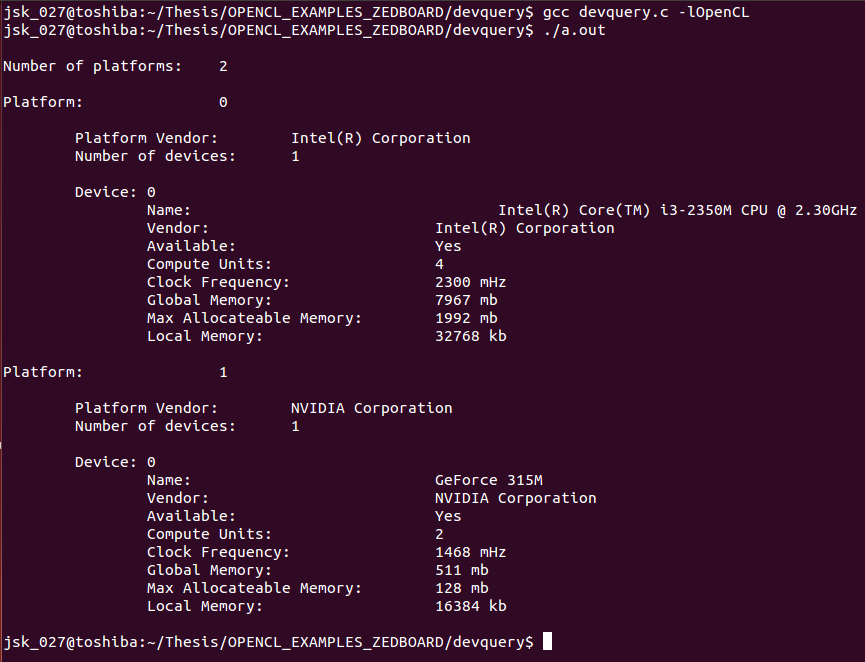
\includegraphics[width=0.7\linewidth]{figures/DeviceQuery.png}
\caption{OpenCL Device Query code Output
\cite{devquery}}
\label{fig:DeviceQuery}
\end{figure}
\subsubsection*{AOCL SDK and Quartus Installation Steps}
The FPGA Implementation of MNIST digit recognition \cite{mnist-altera-opencl} uses Altera OpenCL (AOCL) SDK (also called Intel FPGA SDK) and Quartus Software for high-level synthesis and execution. Although our experiments are not based on the Altera Platform, we may use this SDK to use some OpenCL Libraries which are independent of the hardware.\newline \newline
Intel FPGA SDK for OpenCL™ can be downloaded from \cite{opencl_fpga_sdk}. The installation steps of AOCL and Quartus from the extracted tarball are detailed in \cite{intel_fpga_guide}. Following the installation, the environment variable \textit{\$ALTERAOCLSDKROOT} is by default set to point to the path where the software was installed. A few more environment variables have to be set to inform the software of the FPGA Board in use and the runtime of the host. If the software was installed in the path, say \underline{\textit{/home/intelFPGA\_pro/17.0/hld/}}, then \textit{echo \$ALTERAOCLSDKROOT} returns the same path where software was installed. 
\begin{scriptsize}
\linuxbash
\begin{lstlisting}
$ export PATH=$ALTERAOCLSDKROOT/bin:$PATH
$ export AOCL_BOARD_PACKAGE_ROOT=/home/intelFPGA_pro/17.0/hld/board/s5_ref
$ export QUARTUS_ROOTDIR=/home/intelFPGA_pro/17.0/quartus/bin
$ export LD_LIBRARY_PATH=$ALTERAOCLSDKROOT/host/linux64/lib:$AOCL_BOARD_PACKAGE_ROOT/linux64/lib:/usr/local/lib:$LD_LIBRARY_PATH
$ source $ALTERAOCLSDKROOT/init_opencl.sh
\end{lstlisting}
\end{scriptsize}
\textit{\$AOCL\_BOARD\_PACKAGE\_ROOT} has to refer to the path of the FPGA Board in use. \textit{s5\_ref} is a reference platform available with the SDK files. When using a specific platform, the corresponding platform files are downloaded and the path of the files is used as Board Package Root. \newline \newline
The Altera.icd is copied from \textit{\$ALTERAOCLSDKROOT} to\\ \underline{\textit{/etc/OpenCL/vendors}} and the host application is linked to the ICD Loader using the following lines in the Makefile of the host.
\begin{scriptsize}
\linuxbash
\begin{lstlisting}
AOCL_LDFLAGS=$(shell aocl ldflags)
AOCL_LDLIBS=$(shell aocl ldlibs)

host_prog : host_prog.o
g++ -o host_prog host_prog.o $(AOCL_LDFLAGS) -lOpenCL $(AOCL_LDLIBS)
\end{lstlisting}
\end{scriptsize}

\subsubsection{Existing Code Flow Description}
\label{3_1_3_2}
\begin{figure}[h!]
\centering
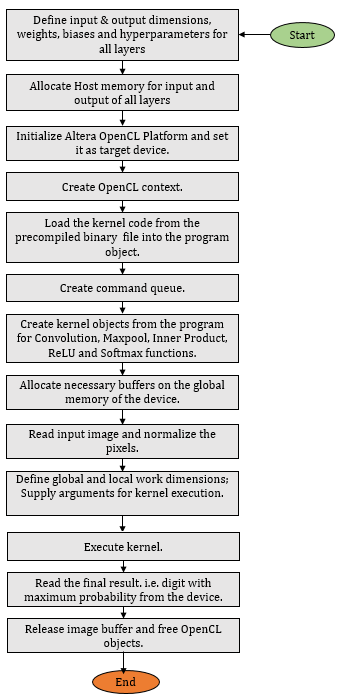
\includegraphics[width=0.5\linewidth]{figures/opencl_flow_lenet5.png}
\caption{OpenCL code flow for Sample (single image recognition) mode \cite{mnist-altera-opencl}}
\label{fig:opencl_flow_lenet5}
\end{figure}
The OpenCL implementation of MNIST/Lenet-5 architecture available in the repository \cite{mnist-altera-opencl} is specific to Altera FPGA devices. In order to make this implementation generic and executable on CPU and GPU, the existing code flow has been examined. Figure \ref{fig:opencl_flow_lenet5} shows the sequence of steps that are done when the a sample image has to be identified.\newline \newline
The first step is the initialization of parameters for all layers in the CNN. This is followed by allocation of buffers necessary for storing inputs and outputs of all layers on the global memory of the device, which is also accessible by the host. The function \textit{ findPlatform()} searches for relevant strings such as Intel FPGA SDK for OpenCL, Altera SDK, etc. When a match-word "Altera" is given as argument to this function, it looks for an Altera platform. Should the platform be available, the next step is to query all OpenCL devices in this platform and set one of them as the target device. \newline\newline
The OpenCL Runtime Environment requires a \textbf{context} to manage memory, program, command issue, kernels, and program execution on the device for which the context is defined. Following the context creation, the source code to be ported to GPU is read into a program object.\newline\newline
There are two ways to compile a kernel \cite{opencl_book_html}. \textbf{Online compilation} involves reading of the kernel source code by the host and building of the source code at runtime by the OpenCL Runtime library. For this, the API \textit{clCreateProgramWithSource()} is used, followed by the API \textit{clBuildProgram()}. This method is not recommended for embedded systems which serve real-time applications. If the kernel is pre-compiled using an OpenCL compiler, the kernel binary is already available and is directly read by the host program, skipping the runtime compilation. This is called \textbf{Offline compilation} and requires only one OpenCL function \textit{clCreateProgramWithBinary()}. Although this saves the time to compile the kernel source during runtime, it is platform-specific. If the same kernel code is to be offloaded to other platforms, then a different set of binaries should be generated. Inclusion of multiple kernel binaries increases the size of the executable.
\begin{figure}[h!]
\centering
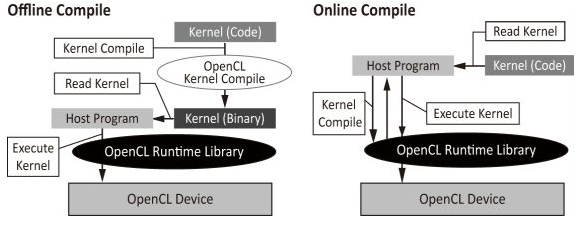
\includegraphics[width=0.7\linewidth]{figures/kernel_compilation.PNG}
\caption{Kernel Compilation Modes \cite{opencl_book_html}}
\label{fig:kernel_compilation}
\end{figure}
The reference code \cite{mnist-altera-opencl} is specific to Altera devices and hence uses offline compilation flow, due to the availability of pre-compiled binary.\newline\newline
Next, a \textbf{command queue} is created which instructs which command has to be executed in which device of the group of devices in a particular context. It also dictates whether the execution should occur in-order or out-of-order. Because the intention is to accelerate the entire ConvNet, kernel objects are created for Convolution, Maxpooling, Inner Product and Activation Layers (ReLU and Softmax). Enough memory has to allocated on the OpenCL device to support the weights, biases and IO dimensions and execution of kernel calls for all 8 layers of the Lenet-5 Model. \newline\newline
The input image pixels are read and normalized. The kernel code is executed on the device after the kernel arguments are supplied to all layers. The final result, i.e. the digit with maximum likelihood is read from the device, buffers and memory objects freed.
\subsubsection{Modifications to remove Platform Dependencies}
\label{3_1_3_3}
\textbf{Allocation of Buffers on the Device Memory:}\newline
For Altera FPGAs, the Altera Offline Compiler (AOC) is responsible for generation of logic to support memory accesses \cite{alteraopencl}. 
\begin{figure}[h!]
 \centering
 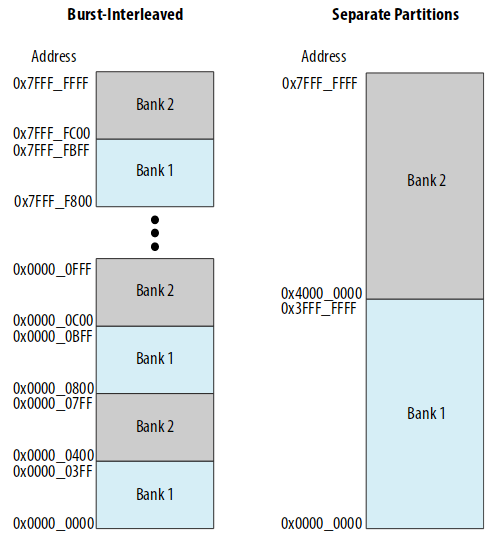
\includegraphics[width=0.5\linewidth]{figures/global_mem_partitions.png}
 \caption{Default (bus-interleaved) vs. Manual Global Memory Partitioning
 \cite{alteraopencl}}
 \label{fig:global_mem_partitions}
\end{figure}
It uses the device SDRAM as global memory and by default, stores the data in a burst-interleaved fashion across various external memory banks. Although this offers uniform load distribution and better balance between the banks, manual partitioning of the data may come in handy for certain applications. For example, when the memory banks support different data-types, data cannot be impartially interleaved to these banks. \newline \newline
The code \cite{mnist-altera-opencl} accesses global memory using optimized memory banks instead of default burst data allocation in the global memory. 
For efficient global memory access, the weights and biases are stored in Bank 2 while the data is stored in Bank 1. However, the memory banks in the GPU context refer to partitioning of shared memory into equal blocks which can be accessed simultaneously. Bank conflicts due to certain access patterns can slow down the GPU performance \cite{gpu_mem_bank}. Hence, the first step to removing platform dependencies is removal of flags CL\_MEM\_BANK\_1\_ALTERA and CL\_MEM\_BANK\_2\_ALTERA which characterize Altera memory banks (Refer \ref{cnncode1:altera-dep-removal}).\newline \newline
\definecolor{hg}{rgb}{0.75,1.0,0.75}
\definecolor{hr}{rgb}{1.0,0.92,0.8}
\newcommand{\grn}{\makebox[0pt][l]{\color{hg}\rule[-4pt]{0.9\linewidth}{10pt}}}
\newcommand{\rd}{\makebox[0pt][l]{\color{hr}\rule[-4pt]{0.9\linewidth}{10pt}}}
\lstset { %
	language=C,
	backgroundcolor=\color{white},
	basicstyle=\ttfamily\tiny,
	keywordstyle=\color{magenta}\ttfamily,
	stringstyle=\color{blue}\ttfamily,
	commentstyle=\color{green}\ttfamily,
    breakatwhitespace=false,
	breaklines=true,
    showstringspaces=false, 
    escapeinside={<@}{@>}
}
\noindent\begin{minipage}{.45\textwidth}
\begin{lstlisting}[caption=Header files for Altera FPGA,frame=tlrb]{Name}
#include <stdio.h>
#include <stdlib.h>
#include <iostream>
#include <iomanip>
#include <fstream>
#include <unistd.h>
#include <math.h>
<@\textcolor{red}{\textbf{\#include "CL/opencl.h"}}@>
<@\textcolor{red}{\textbf{\#include "AOCLUtils/aocl\_utils.h}}@>
#include "cnn_structs.h"
#include "pgm.h"
#include "lenet5_model.h"

<@\textcolor{red}{\textbf{using namespace aocl\_utils;}}@>
using namespace std;
\end{lstlisting}
\end{minipage}\hfill
\begin{minipage}{.45\textwidth}
\begin{lstlisting}[caption=Header files for \\ GPU,frame=tlrb]{Name}
#include <stdio.h>
#include <stdlib.h>
#include <iostream>
#include <iomanip>
#include <fstream>
#include <unistd.h>
#include <math.h>
<@\textcolor{green}{\textbf{\#include <CL/cl.h>}}@>
<@\textcolor{green}{\textbf{\#include <CL/cl\_ext.h>}}@>
#include "cnn_structs.h"
#include "pgm.h"
#include "lenet5_model.h"

using namespace std;
\end{lstlisting}
\end{minipage}\newline
\textbf{Usage of Generic OpenCL headers} \newline
Although AOCL Utility is a platform independent C++ header file, it has been replaced with standard OpenCL headers for the sake of generality. All APIs in the scope of AOCL Utility namespace are substituted by general OpenCL APIs described in \cite{opencl_khronos}. \newline \newline
\textbf{Kernel Loading Mechanism}\newline
On-the-fly kernel loading, i.e. Online compilation method explained in subsection \ref{3_1_3_2} is employed. The existing and modified code changes are depicted clearly in \ref{cnncode3:altera-opencl-init}, \ref{cnncode4:gpu-opencl-init} and \ref{cnncode2:load-kernel-source}.\newline \newline
\textbf{Changes to Makefile}\newline
\textit{libOpenCL.so} Shared Library is linked in the Makefile as shown in Figure \ref{fig:makefile}. Altera platform specific libraries are unlinked.\newline \newline
The resultant code is free of any dependencies with Altera platform and hence, can be compiled and run on any OpenCL device.
\begin{figure}[h!]
\centering
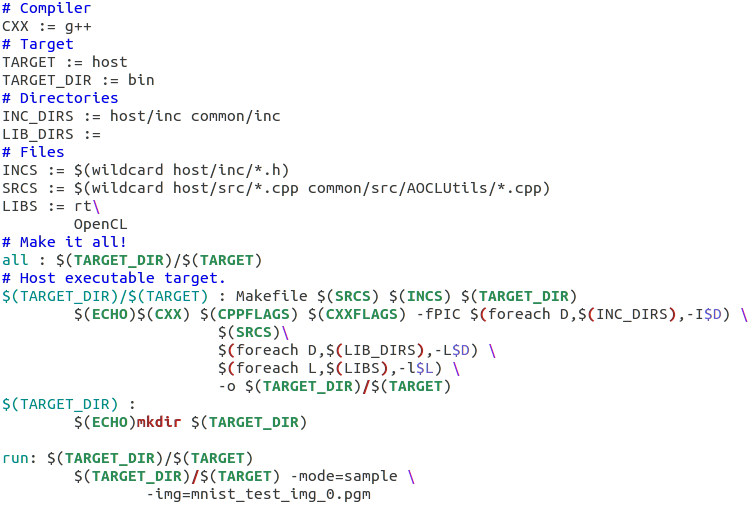
\includegraphics[width=0.7\linewidth]{figures/makefile.png}
\caption{Linking libOpenCL Library to Makefile}
\label{fig:makefile}
\end{figure}
\subsubsection{Compiling and executing the code}
\label{3_1_3_4}
\underline{To test a sample image:}\newline
\begin{scriptsize}
\linuxbash
\begin{lstlisting}
$ make run
\end{lstlisting}
\end{scriptsize}
\underline{To test the full MNIST Dataset:}\newline
\begin{scriptsize}
\linuxbash
\begin{lstlisting}
$ make test
\end{lstlisting}
\end{scriptsize}
The path of the test images (sample and full dataset) is also supplied to the host through the Makefile. Hence, the path has to be suitably modified to point to the test images in the local machine.\newline\newline
The kernels can be executed either in CPU or GPU devices which support OpenCL.\newline
\hfill
\begin{minipage}{\textwidth}
\begin{center}
\begin{lstlisting}[caption= CPU or GPU Device Selection,frame=tlrb]{Name}
int gpu = 1;
for(unsigned i = 0;i < dev_cnt; i++){
   err = clGetDeviceIDs(platform_ids[i], gpu ? CL_DEVICE_TYPE_GPU : CL_DEVICE_TYPE_CPU, 1, &target_device, NULL);
   if(err == CL_SUCCESS){
      break;
   }
}
\end{lstlisting}
\end{center}
\end{minipage}
When the integer variable \textit{'gpu'} is set to 1, the GPU device is selected and when it is set to 0, the CPU device is selected.
\subsubsection*{Benchmarking Kernel Execution Time}
\begin{itemize}
\item Profiling should be enabled during the creation of command queue as follows:\\
\begin{minipage}{\textwidth}
\begin{center}
\begin{lstlisting}[columns=fullflexible, language=C++, escapechar = \$, backgroundcolor=\color{gray!10}]
queue = clCreateCommandQueue(context, target_device, $\textcolor{red}{CL\_QUEUE\_PROFILING\_ENABLE}$, &status); 
checkError(status, "Failed to create command queue");
\end{lstlisting}
\end{center}
\end{minipage}
\item An event is associated with the kernel during its launch as follows:\\
\begin{minipage}{\textwidth}
\begin{center}
\begin{lstlisting}[columns=fullflexible, language=C++, escapechar = \$, backgroundcolor=\color{gray!10}]
status = clEnqueueNDRangeKernel(queue, kernel[0], 3, NULL, global_work_size, NULL, 0, NULL, $\textcolor{red}{\&kernel\_event[0]}$);
checkError(status, "Failed to launch conv1 kernel");
\end{lstlisting}
\end{center}
\end{minipage}
\item Kernel execution has to be completed and also all enqueued tasks in the command queue should finish.\\
\begin{minipage}{\textwidth}
\begin{center}
\begin{lstlisting}[columns=fullflexible, language=C++, escapechar = \$, backgroundcolor=\color{gray!10}]
clWaitForEvent(1, &kernel_event[0]);
clFinish(queue);
\end{lstlisting}
\end{center}
\end{minipage}
\item The following APIs can be used to estimate the kernel execution time:\\
\begin{minipage}{\textwidth}
\begin{center}
\begin{lstlisting}[columns=fullflexible, language=C++, escapechar = \$, backgroundcolor=\color{gray!10}]
cl_ulong start_time, end_time;
double total_time;
clGetEventProfilingInfo(kernel_event[0], CL_PROFILING_COMMAND_START, sizeof(start_time), &start_time, NULL);
clGetEventProfilingInfo(kernel_event[0], CL_PROFILING_COMMAND_END, sizeof(end_time), &end_time, NULL);
total_time = end_time-start_time;
printf("Kernel Execution Time is: %0.3f \n",total_time/1000000.0);
\end{lstlisting}
\end{center}
\end{minipage}
\end{itemize}
\subsection{Comparative Study of Results}
\label{3_1_4}
\textbf{Test Devices}
\begin{enumerate}
\item \textbf{Intel OpenCL} from Intel(R) Corporation \\
OpenCL Version: OpenCL 1.2 LINUX\\
Compute Units: 4
\item \textbf{NVIDIA CUDA} from NVIDIA Corporation\\ 
OpenCL Version: OpenCL 1.1 CUDA 4.2.1\\
Compute Units:2
\end{enumerate}
\newcolumntype{L}[1]{>{\raggedright\arraybackslash}p{#1}}
\begin{table}[htbp]
\caption{Comparison of kernel runtime in various OpenCL Devices}
\centering
\begin{tabular}{@{}p{0.25\textwidth}*{2}{L{\dimexpr0.22\textwidth-2\tabcolsep\relax}}@{}}
\toprule
& \multicolumn{2}{c}{Kernel Execution Time (ms)} \\
\cmidrule(r{4pt}){2-3} & Intel Core i3-2350M CPU @ 2.30GHz (4 CUs) & NVIDIA GeForce 315M (2 CUs)\\
\midrule
Convolution 1 & \makecell[c]{0.216} & \makecell[c]{0.707}\\
\midrule
MaxPool 1 &\makecell[c]{0.046} &\makecell[c]{0.166} \\
\midrule
Convolution 2 &\makecell[c]{0.716} &\makecell[c]{11.332} \\
\midrule
Maxpool 2 &\makecell[c]{0.026} &\makecell[c]{0.371} \\
\midrule
Inner Product 1&\makecell[c]{0.187} &\makecell[c]{1.651} \\
\midrule
ReLU &\makecell[c]{0.011} &\makecell[c]{0.012} \\
\midrule
Inner Product 2&\makecell[c]{0.010} &\makecell[c]{0.287} \\
\midrule
Softmax &\makecell[c]{0.014} &\makecell[c]{0.012} \\
\bottomrule
\end{tabular}
\label{table:results_compare_cnn}
\end{table}

\textbf{Goal:} The ratio $R_{acceleration}$ = $\frac{t_{sw}}{t_{hw}} \>$ 1\newline \newline
Device 1: $R_{acceleration}$ = $\frac{0.077}{1.30224 \times 10^{-3}}$ = 59.12\newline \newline
Device 2: $R_{acceleration}$ = $\frac{0.077}{16.09 \times 10^{-3}}$ = 4.78
\chapter{Hardware Acceleration using FPGA}
\label{ch4_fhew}

\section{Fully Homomorphic Encryption Scheme}
\label{4_1}
Fully Homomorphic Encryption scheme allows computation of arithmetic or logical functions on encrypted data, without decrypting them. It was first conceptualized and realized by Craig Gentry in 2009 \cite{gentry2010computing}.  Several improvements have been made since then to improve the security of the initial scheme \cite{gentry2011implementing}\cite{gentry2012homomorphic}\cite{halevi2014algorithms} and to make the number of homomorphic operations asymptotically large, by reducing the noise in ciphertexts. \textit{Bootstrapping} is a novel method introduced by Gentry to reduce noise in ciphertexts to acceptable levels, by homomorphically evaluating the decryption function using the encrypted secret key. However, Bootstrapping is a costly operation \cite{ducas2015fhew} and takes around 0.69 seconds in software. This brings in some motivation for hardware acceleration, to achieve a practical performance.\newline\newline
To offload the FHE operations to hardware, it is important to have some mathematical awareness and understanding of the various steps involved in FHE. The paper \cite{ducas2015fhew} introduces the library, FHEW \cite{fhew_lib} which performs a simple Bootstrapped NAND operation exhibiting lower noise levels compared to previous FHE schemes discussed in \cite{halevi2014algorithms}\cite{gentry2012homomorphic}. This method is not restricted to NAND operation but can be extended to various other arithmetic and logical computations \cite{ducas2015fhew}. \newline
The Figure \ref{fig:fhew_prob_stmt} illustrates the problem statement that we seek to address through this scheme. One practical application of this scheme is to delegate data-processing to the cloud without giving away the original data. 
\begin{figure}[h!]
 \centering
 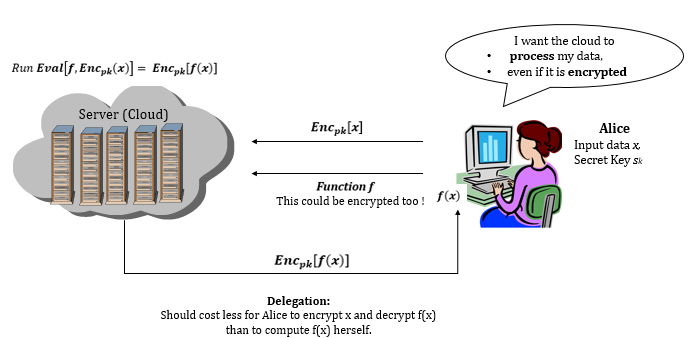
\includegraphics[width=\linewidth]{figures/fhew_prob_stmt.PNG}
 \caption{FHE: Problem Statement
 \cite{shai_he}}
 \label{fig:fhew_prob_stmt}
\end{figure}
\subsection{Background}
\label{4_1_1}
\subsubsection*{Homomorphism}
Given two groups, G and H, Homomorphism from G to H can be defined as a function \textit{f: $G \rightarrow H$}, such that:
\begin{adjustwidth}{2cm}{}
f($g_1$ * $g_2$) = f($g_1$) * f($g_2$), \\
$g_1$, $g_2$ : Elements in \textit{G},\\
* : Operation in \textit{G}, \\
* : Operation in \textit{H}
\end{adjustwidth}
\subsubsection*{Steps in FHE}
Fully homomorphic encryption scheme $\epsilon$ has 4 key steps:\\
1. $KeyGen_\epsilon$($\lambda$)\\
It involves generation of random secret key, which is an odd integer \textit{p}, P-bits long. The security parameter $\lambda$ dictates the bit-length of the key.
\begin{itemize}
\item Symmetric Encryption: \\
Encryption and Decryption are performed using the same secret key.  
\item Asymmetric Encryption:\\ Encryption is done using a public key ($p_k$) and Decryption using a secret key ($s_k$).
\end{itemize}
2. $Encrypt_\epsilon$(\textit{p,m})\\
Given the security parameter $\lambda$, 
\begin{adjustwidth}{2cm}{}
N = $\lambda$; P = $\lambda^2$; Q = $\lambda^5$
\end{adjustwidth}
\underline{Scheme \cite{gentry2010computing}:}\\
To encrypt a bit \textit{m} $\in$ \{0,1\}, set \textit{m'= m mod 2}, a random N-bit number.
\begin{adjustwidth}{2cm}{}
Output ciphertext: \textit{c $\leftarrow$ m' + pq},
\end{adjustwidth}
where \textit{q} is a random Q-bit integer.
\begin{adjustwidth}{2cm}{}
i.e. \textit{c $\leftarrow$ m mod 2 + pq}
\end{adjustwidth}
3. $Decrypt_\epsilon$(\textit{p,c})
\begin{adjustwidth}{2cm}{}
Output: \textit{c' mod 2}, 
\end{adjustwidth}where \textit{c' = c mod p} is an integer in the range \textit{(-p/2, p/2)} and \textit{p} divides \textit{c-c'}.\\
\textit{c - c' = c - c mod p = c (1 - mod p)} is divisible by \textit{p}. Hence, the ciphertexts of $\epsilon$ are near-multiples of \textit{p}.\\
To maintain a constant complexity for decryption, any two ciphertexts $c_1$ and $c_2$ outputted from the encryption scheme should be of the same size \cite{gentry2010computing}. Size of the ciphertext and the time taken to decrypt should be independent of the complexity of function \textit{f}, delegated to the cloud.\newline\newline
4. $Evaluate_\epsilon$(\textit{$p_k$, f, $c_1$, $c_2$, ... $c_t$})\\For any function \textit{f} in a set of permissible functions \textit{$F_\epsilon$}, and ciphertexts \textit{$c_1$, $c_2$... $c_t$}, where \textit{$c_i$} $\leftarrow$ \textit{$Encrypt_\epsilon$}(\textit{$p_k$, $m_i$}), the following 2 steps are performed:
\begin{adjustwidth}{2cm}{}
\textit{c} $\leftarrow$ \textit{$Encrypt_\epsilon$[ f ($c_1$, $c_2$, ... $c_t$)]}\\
$Decrypt_\epsilon$(c , $s_k$) = \textit{f ($m_1$, $m_2$, ... $m_t$)}
\end{adjustwidth}
\begin{figure}[h!]
 \centering
 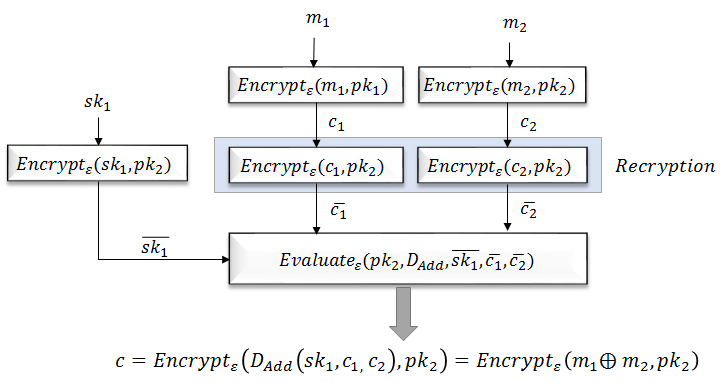
\includegraphics[width=\linewidth]{figures/Eval_FHE.png}
 \caption{Homomorphic Encryption Scheme : Example
 \cite{gentry2010computing}}
 \label{fig:Eval_FHE}
\end{figure}
This scheme guarantees one-wayness and semantic security against chosen plain-text attacks, as it is probabilistic \cite{gentry2010computing}. Figure \ref{fig:Eval_FHE} shows 2 messages $m_1$ and $m_2$ encrypted using public key $pk_1$ whose associated secret key is $sk_1$. $Evaluate_\epsilon$ takes in the resultant ciphertexts $c_1$, $c_2$ and secret key $sk_1$ encrypted under another key $pk_2$ and outputs \textit{c} which is an encryption of $D_\epsilon$ result under $pk_2$.
\subsubsection*{Concept of Bootstrapping}
\begin{figure}[h!]
 \centering
 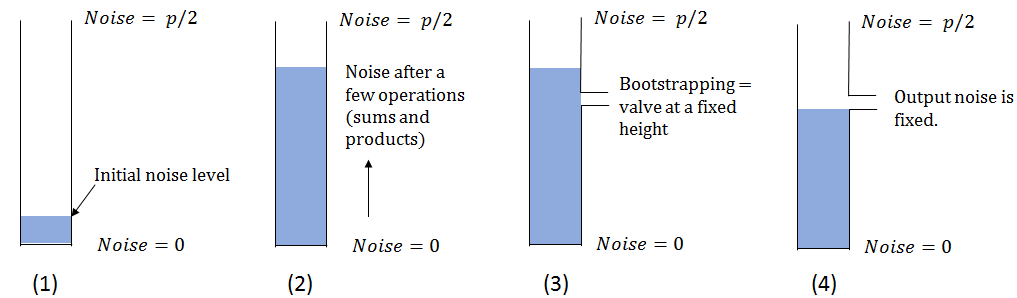
\includegraphics[width=\linewidth]{figures/bootstrapping.png}
 \caption{Homomorphic Decryption: Example
 \cite{he_utoronto}}
 \label{fig:bootstrapping}
\end{figure}
Decryption reduces the noise. However, decrypting the data in remote server can compromise security. So, homomorphic decryption described in Figure \ref{fig:Eval_FHE} is used to reduce the noise level, so that the result is decipherable at the receiver. 
\subsection{Existing code flow}
\label{4_1_1}
\begin{figure}[h!]
 \centering
 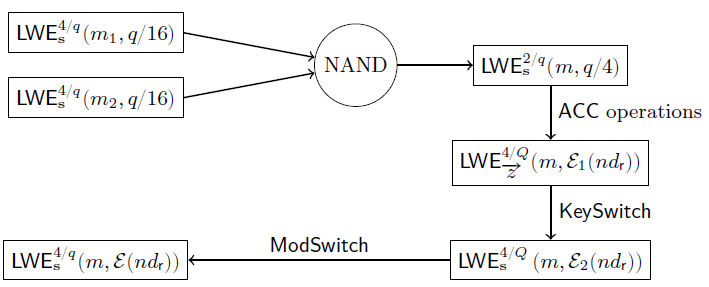
\includegraphics[width=0.8\linewidth]{figures/FHEW.PNG}
 \caption{Cycle of simple NAND operation
 \cite{ducas2015fhew}}
 \label{fig:FHEW}
\end{figure}
The FHEW Library \cite{fhew_lib} uses the ring lattice for encryption and bootstrapping, to reduce the computation time to quasi-linear complexity (Using FFT) as opposed to the quadratic complexity of previous methods \cite{ducas2015fhew}.\newline\newline
The \textit{Learning With Errors} (LWE) encryption scheme has been used to generate ciphertexts, with a message modulus of 4 and error bound of q/16. The specifics of this scheme have been described in great detail in \cite{ducas2015fhew} for further reading, and shall not be covered in this thesis. A random evaluation key, constituting a bootstrapping key and switching key is generated for a given LWE secret key. Both encryption and recryption (Figure \ref{fig:Eval_FHE}) use the LWE scheme but with different keys. Two ciphertexts LWE-encrypted using a n-dimensional secret key (n = 500) are fed to the Homomorphic NAND block:\newline \newline
HomNAND: $LWE_{s}^\frac{4}{q}$($m_0$, q/16) x $LWE_{s}^\frac{4}{q}$($m_1$, q/16)$\rightarrow$ $LWE_{s}^\frac{2}{q}$($m_0 \bar{\wedge} m_1$, q/4)\newline \newline
where LHS denotes ciphertext inputs encrypting binary messages, $m_0, m_1$ $\in$ \{0,1\} with error limit as q/16. RHS is the HomNAND output which is an encryption of the logical NAND of the two input messages = 1 - $m_0.m_1$ = $m_0 \bar{\wedge} m_1$, with an error bound of q/4.
The switching key facilitates conversion of LWE encryption with one secret key to another LWE encryption using a different secret key. Modulus switching helps switch the LWE ciphertexts from one modulus (Q) to another (q). \\The most efficient Bootstrapping method proposed by the author is the one using FFTs (Section 5.3, \cite{ducas2015fhew}). The Fastest Fourier Transform in the West (FFTW) Library \cite{FFTW05} is an open-source benchmark library for optimized software FFT computations. This library has been used for performing FFTs and inverse FFTs in the FHE algorithm, with double-precision floating point accuracy. 
\subsection{Hot-Spots for Hardware Acceleration}
\label{4_1_2}
One major difference in FPGA programming, be it RTL or HLS, is the bit-width precision. Register sizes are deterministic at compile time. Libraries such as $<ap\_cint.h>$ and $<ap\_int.h>$ in Vivado HLS facilitate specification of bit-accurate variables.  We notice that FFTW Library required by FHEW library is compiled for double-precision floating point accuracy which is 64-bits long by default. Usually, Embedded devices are memory and power constrained. Hence, exploring the accuracy of results with varying bit-widths is another interesting aspect to investigate, for a holistic analysis of hardware acceleration using FPGAs.\\
Software Profiling results have confirmed that the Homomorphic NAND operation takes up the maximum execution time. Each HomNAND operation makes several calls to Accumulator as illustrated in Table \ref{table:sw_hotspots_fhe}. The accumulator in turn calls the 2048-point FFT and IFFT routines several times.
\begin{table}[htbp]
\caption{Analysis of Software Bottlenecks}
\centering
\begin{tabular}{c p{4.5cm} c}
\toprule
HomNAND Test Count & Function & Number of function calls\\
\midrule
\multirow{4}{*}{0}&FFT&396002\\
\cmidrule(r{4pt}){2-3}
  &Inverse FFT&132000\\
\cmidrule(r{4pt}){2-3}
 &Homomorphic NAND&0\\
\cmidrule(r{4pt}){2-3}
 &Add to Accumulator&0\\
\midrule
\multirow{4}{*}{1}&FFT&499430\\
\cmidrule(r{4pt}){2-3}
 &Inverse FFT&166470\\
\cmidrule(r{4pt}){2-3}
 &Homomorphic NAND&3\\
\cmidrule(r{4pt}){2-3}
 &Add to Accumulator&2872\\
\bottomrule
\end{tabular}
\label{table:sw_hotspots_fhe}
\end{table}
The tabulated values are averages obtained from 5 runs of the application in each of the two cases, HomNAND Test for 0 and 1 rounds. The number of function calls is not deterministic but usually around a certain range, due to the random nature of input, secret and bootstrapping keys. Each HomNAND Test involves 3 HomNAND function calls in the implemented FHE design \cite{fhew_lib} \ref{table:sw_hotspots_fhe}. This is because the circuit under test is defined by: (\textbf{a} NAND \textbf{b}) NAND (\textbf{c} NAND \textbf{d}).
\subsubsection{Dimensionality Analysis}
\begin{table}[]
\centering
\caption{Dimensionality Analysis (Section 6.2, \cite{ducas2015fhew})}
\label{tab:fhew_dim}
\begin{tabular}{@{}m{0.5\linewidth} m{0.5\linewidth}@{}}
\toprule
\multicolumn{1}{c}{\textbf{Parameter}} & \multicolumn{1}{c}{\textbf{Size}} \\ \midrule
\multicolumn{1}{l}{LWE Secret Key} & \multicolumn{1}{l}{Array of size 500} \\ \midrule
\multicolumn{1}{l}{\multirow{2}{*}{Evaluation Key}} & \multicolumn{1}{l}{BootstrappingKey{[}500{]}{[}23{]}{[}2{]}} $\approx$ 1032 MBytes \\ \cmidrule(l){2-2} 
\multicolumn{1}{l}{} & \multicolumn{1}{l}{SwitchingKey{[}1024{]}{[}25{]}{[}7{]} $\approx$ 314 MBytes} \\ \midrule
\multicolumn{1}{l}{HomNAND Inputs} & \multicolumn{1}{l}{1-bit} \\ \midrule
\multicolumn{1}{c}{\multirow{2}{*}{\begin{tabular}[c]{@{}c@{}}HomNAND Output Cipher\\ (a,b);\end{tabular}}} & \multicolumn{1}{l}{\begin{tabular}[c]{@{}l@{}}a{[}500{]} - coefficient vector over a \\ cyclotomic ring R in Z{[}X{]}/$X^N$+1;\end{tabular}} \\ \cmidrule(l){2-2} 
\multicolumn{1}{c}{} & \multicolumn{1}{l}{b = \textbf{a.s} + e, where e is the error.} \\ \midrule
\multicolumn{1}{l}{Decrypt Output} & \multicolumn{1}{l}{32 bits} \\ \bottomrule
\end{tabular}
\end{table}
Table \ref{tab:fhew_dim} shows the dimensions of the inputs, intermediate values, secret keys and output in the encryption scheme. The bootstrapping and switching keys used in AddToAccumulator block of HomNAND operation are of huge sizes and hence, replicating multiple AddToAccumulator blocks in the hardware could be costly, without prior optimizations. Table \ref{table:sw_hotspots_fhe} shows that each Homomorphic NAND test involves around $\frac{499430 - 396002}{3}$ = 34476 FFT operations and the author confirms in Section 6.2, \cite{ducas2015fhew} that as high as 48000 FFTs are performed per NAND gate. 
\begin{table}[htbp]
\caption{Software Computation Time}
\centering
\begin{tabular}{l c}
\toprule
\textbf{Operation} & \textbf{Computation Time ($\mu$s)}\\
\midrule
FFTW FFT &30.892\\
\midrule
FFTW IFFT &23.93\\
\bottomrule
\end{tabular}
\label{table:fft_time}
\end{table}
The Table \ref{table:fft_time} illustrates the average execution time of a single FFT and IFFT, taken across 500 readings in a quad-core CPU. Since the speed of the algorithm depends on the speed of FFTs, porting this portion to hardware helps achieve a faster execution. We observe that FFTW is highly efficient in terms of runtime in software. However, it is a huge library and not hardware-friendly. \newline \newline
\subsection{Results}
\label{4_1_2}
\subsubsection*{Precision Analysis}
To determine whether double-precision floating point FFT is required to preserve the functionality of FHEW, the source code of FHEW was linked to different precision libraries and output analyzed. The configure script that comes with the library source files is used to generate Makefile. By using different compiler flags \cite{fftw_unix}, the FFTW library can be compiled for:
\begin{itemize}
\item single precision floating point
\begin{scriptsize}
\linuxbash
\begin{lstlisting}
$ sudo ./configure --enable-float
\end{lstlisting}
\end{scriptsize}
\item quadruple-precision floating point (\_\_float128)
\begin{scriptsize}
\linuxbash
\begin{lstlisting}
$ sudo apt-get install libquadmath
$ sudo ./configure --enable-quad-precision
\end{lstlisting}
\end{scriptsize}
\item long double 
\begin{scriptsize}
\linuxbash
\begin{lstlisting}
$ sudo ./configure --enable-long-double
\end{lstlisting}
\end{scriptsize}
\end{itemize}
When no option is specified, the default precision is \textit{double}. The below commands install the library with the new precision settings.
\begin{scriptsize}
\linuxbash
\begin{lstlisting}
$ make
$ make install
\end{lstlisting}
\end{scriptsize}
The source code of FHEW is linked to the new libraries: \textbf{-lfftw3f} (for float) or \textbf{-lfftw3l} (for long double) or \textbf{-lfftw3q -lquadmath -lm} (for quad-float) instead of the default library \textbf{-lfftw3}.\newline\newline
All lower-case instances of "fftw\_" in the FFT function calls and datatypes are replaced by fftwf\_ (for float) or fftl\_ (for long double) or fftwq\_ (for quad-float).\\
\textbf{Example:} The datatype \textbf{fftw\_complex} becomes \textbf{fftwf\_complex} or \textbf{fftwl\_complex} or \textbf{fftwq\_complex }depending on the desired precision.\newline \newline
As our intention is reduction of bit-width, the experiments were based on single-precision and quad-precision float. Upon making the above-mentioned changes, the FHEW functionality was not preserved due to reduction in accuracy. Supporting the analysis, the authors of \cite{ducas2015fhew} have stated that double-precision float is barely sufficient to contain the error levels within an acceptable range (Section 6.3, \cite{ducas2015fhew}). Figure \ref{fig:fft_precision_loss} illustrates the loss of functionality upon linking the source code to a lower precision FFT.
\begin{figure}[h!]
 \centering
 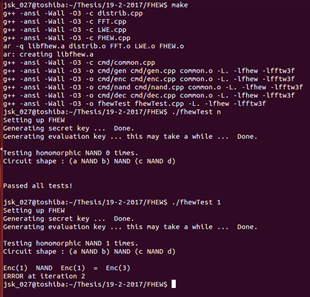
\includegraphics[width=0.5\linewidth]{figures/fft_precision_loss.png}
 \caption{Precision Loss with single-precision float}
 \label{fig:fft_precision_loss}
\end{figure}
From the above experiments, we conclude that of the standard datatypes, \textbf{double} is the lowest allowable precision that preserves the homomorphic encryption functionality. \newline\newline
FFTs can also be performed in integer domain using Number Theoretic Transform library (NTL) used in \cite{helib}. NTL involves convolution of 2 sequences modulo a prime number. Hence, the choice of modulus with respect to sequence length is restricted \cite{bhattacharya2004some}. FFTW has proved to be much more optimized and faster than the latter as stated in Section 6.3, \cite{ducas2015fhew}, which is why FHEW is an improvement over HELib \cite{shai_he} which uses NTL, in terms of Bootstrapping runtime. As the optimization objective is to improve run-time, FFT function can be hand-optimized for hardware acceleration and the functional correctness verified, by integrating with the existing software implementation.
\subsubsection*{FFT Offload}
Various FFT implementations were explored, intuitively optimized and their runtime performance was studied using High-level synthesis tools.
Firstly, the Xilinx FFT IP Core \cite{logicore2012fast} was analyzed and its usage studied. It implements the Cooley Tukey (Radix-4 DIT) FFT and accepts input in full-precision fixed point, scaled fixed point and block floating point . Since double-precision inputs are not supported by this hard block, it is not an ideal candidate for our application's acceleration. Then, a Cooley Tukey FFT algorithm was implemented, of size N given by the product $N_1$.$N_2$ where $N_1$ naive DFTs, each of size $N_2$ were performed. 
\begin{table}[htbp]
\centering
\caption{Execution time of unoptimized Cooley Tukey implementation with transform length N = 1024 in Avnet Zedboard Evaluation Platform}
\label{tab:ct_fft_1}
\begin{tabular}{|c|l|l|l|l|l|}
\hline
\textbf{N1} & 512 & 256 & 128 & 64 & 32 \\ \hline
\textbf{N2} & 2 & 4 & 8 & 16 & 32 \\ \hline
\textbf{Execution Time (s)} & 1.5 & 0.77 & 0.38 & 0.23 & 0.18 \\ \hline
\end{tabular}
\end{table}
From Table \ref{tab:ct_fft_1}, we see that the execution time was in the order of seconds, irrespective of the values of $N_1$ and $N_2$. Thus, this implementation was further improved by doing loop and function optimizations, integrated to the FHEW code and the functional correctness was verified. Taking it further, a radix-2 butterfly DIF FFT logic was implemented. \newline \newline For these implementations to be synthesizable by the high-level synthesis tool, recursive calls and dynamic memory allocation were avoided and all pointers were made deterministic at compile time. Various optimization directives were intuitively chosen to offer improved runtime performance and the best optimization was identified. The pros and cons of all three implementations were studied to decide on which best suits our need.  
\subsubsection{Hand-optimized non-recursive 1-D FFT}
Table \ref{tab: dse_1dfft} illustrates the clock period, latency and utilization estimates upon applying different optimization directives to the hand-optimized FFT implementation for hardware. We observe that solution 4 offers the most optimal area-latency design point. 
\newcolumntype{L}{>{\centering\arraybackslash}p{{0.15\linewidth}}}
\begin{table}[htbp]
\centering
\caption{Design Space Exploration for non-recursive 1-D FFT}
\label{tab: dse_1dfft}
\begin{tabular}{|m{2cm}|m{1.5cm}|L|L|L|L|L|}
\hline
\multicolumn{7}{|c|}{\textbf{Target: Avnet Zedboard Evaluation xc7z020clg484-1}} \\ \hline
\multicolumn{2}{|l|}{} & \textbf{Solution 1} & \textbf{Solution 2} & \textbf{Solution 3} & \textbf{Solution 4} & \textbf{Solution 5} \\ \hline
\multicolumn{2}{|c|}{\textbf{Optimization}} & No directives. & Loop 0: Pipeline& Loop 0: Unroll & Loop 0 \& 2: Pipeline & Loop 0: Pipeline, Loop 2: Unroll \\ \hline
\multicolumn{2}{|c|}{\textbf{\begin{tabular}[c]{@{}c@{}}Estimated\\Clock Period\\(ns)\end{tabular}}} & 9.83 & 9.83 & 12.93 & 11.96 & 12.19 \\ \hline
\multirow{2}{*}{\textbf{\begin{tabular}[c]{@{}c@{}}Latency\\ (cycles)\end{tabular}}} & \textbf{Min} & 295730178 & 295705626 & 297810991 & 5387290 & 8048665 \\ \cline{2-7} 
 & \textbf{Max} & 945847298 & 945822746 & 947928111 & 5387290 & 12492825 \\ \hline
\multirow{4}{*}{\textbf{\begin{tabular}[c]{@{}c@{}}Utilization\\ Estimates\end{tabular}}} & \textbf{BRAM} & 13 & 13 & 13 & 8 & 13234 \\ \cline{2-7} 
 & \textbf{DSP48E} & 67 & 73 & 234 & 105 & 31410 \\ \cline{2-7} 
 & \textbf{FF} & 7235 & 8245 & 149093 & 32308 & 4632256 \\ \cline{2-7} 
 & \textbf{LUT} & 24133 & 26896 & 117748 & 70551 & 19331620 \\ \hline
\end{tabular}
\end{table}

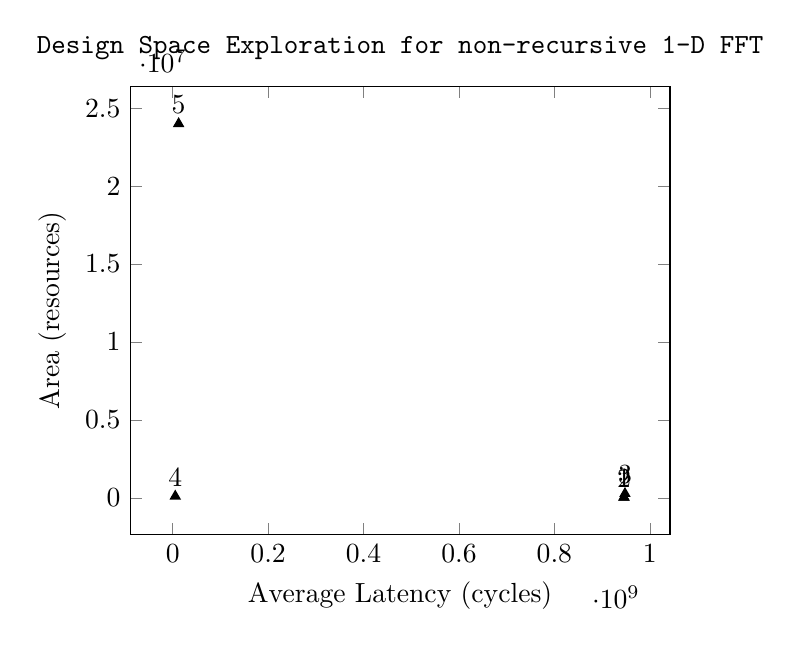
\begin{tikzpicture}
\label{graph:dse_1dfft}
\centering
	\begin{axis}[
		xlabel= Average Latency (cycles),
		ylabel=Area (resources),     
        nodes near coords, % Place nodes near each coordinate
    point meta=explicit symbolic, % The meta data used in the nodes is not explicitly provided and not numeric
	    title={\texttt{Design Space Exploration for non-recursive 1-D FFT}}]        
	\addplot[mark=triangle*, only marks, mark options={fill=black}] 
    table [% Provide data as a table
     meta index=2 % the meta data is found in the third column
     ] {
   x          y     label
945847298    31448    1
945822746    35227    2
947928111   267088    3
5387290     102972    4
12492825  24008520    5
	};
	\end{axis}
\end{tikzpicture}

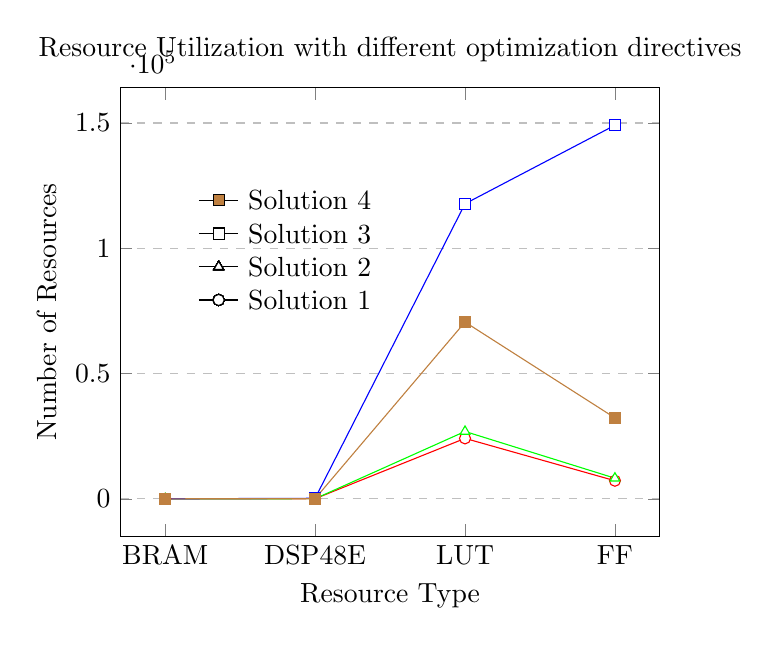
\begin{tikzpicture}
\begin{axis}[
    title={Resource Utilization with different optimization directives},
    xlabel={Resource Type},
    ylabel={Number of Resources},
    xtick=data,    
    legend pos=north west,
    ymajorgrids=true,
    grid style=dashed, 
    symbolic x coords={BRAM, DSP48E, LUT, FF},
]
 
\addplot[
    mark=*, mark options={fill=white}, color = red
    ]
    coordinates {
    (BRAM,13)
    (DSP48E,67)
    (LUT,24133)
    (FF,7235)
    };   

\addplot[
    mark=triangle*, mark options={fill=white}, color = green
    ]
    coordinates {
    (BRAM,13)
    (DSP48E,73)
    (LUT,26896)
    (FF,8245)
    };    
    
\addplot[
    mark=square*, mark options={fill=white}, color = blue
    ]
    coordinates {
    (BRAM,13)
    (DSP48E,234)
    (LUT,117748)
    (FF,149093)
    };    
    
\addplot[
    mark=square*, mark options={fill=brown}, color = brown
    ]
    coordinates {
    (BRAM,8)
    (DSP48E,105)
    (LUT,70551)
    (FF,32308)
    };    
\end{axis}    
    \begin{scope}[shift={(1,3)}] 
	\draw (0,0) -- 
		plot[mark=*, mark options={fill=white}, color=red] (0.25,0) -- (0.5,0) 
		node[right]{Solution 1};
	\draw[yshift=\baselineskip] (0,0) -- 
		plot[mark=triangle*, mark options={fill=white}, color=green] (0.25,0) -- (0.5,0)
		node[right]{Solution 2};
	\draw[yshift=2\baselineskip] (0,0) -- 
		plot[mark=square*, mark options={fill=white}, color=blue] (0.25,0) -- (0.5,0)
		node[right]{Solution 3};
	\draw[yshift=3\baselineskip] (0,0) -- 
		plot[mark=square*, mark options={fill=brown}, color = brown] (0.25,0) -- (0.5,0)
		node[right]{Solution 4};
	\end{scope}

\end{tikzpicture}

\subsubsection{Cooley Tuckey Radix-2 DIF FFT}
DIF FFT takes inputs in bit-reversed order and produces outputs in natural order. Shift operators are used instead of the costly multipliers. This implementation is in-place to reduce migration costs and less intuitive, but better optimized for hardware. \newline\newline
Appendix \ref{fhewcode3:CTfft} shows that some loop bounds are not statically defined. So, the HLS tool cannot determine the number of iterations of a variable-length loop at runtime and hence, cannot supply the latency estimates. To circumvent this problem, the directive "Loop Trip Count" is applied by manually specifying the maximum number of times this loop will be executed, at compile time.\newline\newline

\begin{table}[htbp]
\centering
\caption{Design Space Exploration for Cooley Tukey Radix-2 DIF FFT}
\label{tab:dse_ctfft}
\begin{tabular}{|m{2cm}|m{1.5cm}|L|L|L|L|}
\hline
\multicolumn{6}{|c|}{\textbf{Target: Avnet Zedboard Evaluation xc7z020clg484-1}} \\ \hline
\multicolumn{2}{|l|}{} & \textbf{Solution 1} & \textbf{Solution 2} & \textbf{Solution 3} & \textbf{Solution 4} \\ \hline
\multicolumn{2}{|c|}{\textbf{Optimization}} & \begin{tabular}[c]{@{}c@{}}Loops 1,2:\\Trip\\Count \\= 512\end{tabular} & \begin{tabular}[c]{@{}c@{}}Loops 1,2:\\Trip\\Count \\= 512,\\Loop 3:\\Pipeline\end{tabular} & \begin{tabular}[c]{@{}c@{}}Loops 1,2:\\Trip\\Count \\= 512,\\ Loop 3:\\Unroll\end{tabular} & \begin{tabular}[c]{@{}c@{}}Loops 1,2:\\Trip\\Count \\= 512,\\ Loop 3:\\Unroll\\(factor 16)\end{tabular} \\ \hline
\multicolumn{2}{|c|}{\textbf{Estimated Clock Period}} & 8.23 & 8.23 & 8.23 & 8.23 \\ \hline
\multirow{2}{*}{\textbf{\begin{tabular}[c]{@{}c@{}}Latency\\ (cycles)\end{tabular}}} & \textbf{Min} & 2170 & 3195 & 1112 & 1210 \\ \cline{2-6} 
 & \textbf{Max} & 49871994 & 49871995 & 49869912 & 49871994 \\ \hline
\multirow{4}{*}{\textbf{\begin{tabular}[c]{@{}c@{}}Utilization\\ Estimates\end{tabular}}} & \textbf{BRAM\_18K} & 0 & 0 & 0 & 0 \\ \cline{2-6} 
 & \textbf{DSP48E} & 56 & 56 & 56 & 56 \\ \cline{2-6} 
 & \textbf{FF} & 4511 & 4513 & 131834 & 6996 \\ \cline{2-6} 
 & \textbf{LUT} & 8529 & 8529 & 67506 & 9932 \\ \hline
\end{tabular}
\end{table}

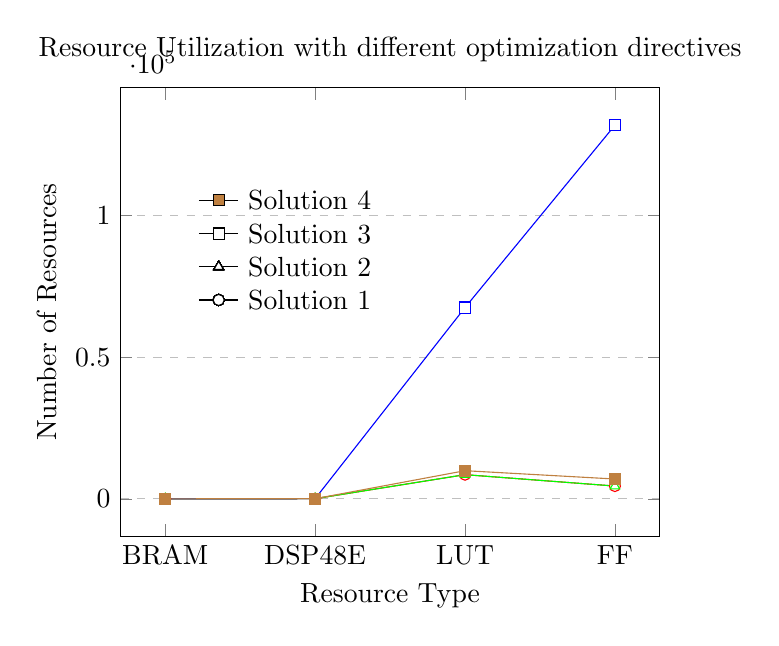
\begin{tikzpicture}
\begin{axis}[
    title={Resource Utilization with different optimization directives},
    xlabel={Resource Type},
    ylabel={Number of Resources},
    xtick=data,    
    legend pos=north west,
    ymajorgrids=true,
    grid style=dashed, 
    symbolic x coords={BRAM, DSP48E, LUT, FF},
]
 
\addplot[
    mark=*, mark options={fill=white}, color = red
    ]
    coordinates {
    (BRAM,0)
    (DSP48E,56)
    (LUT,8529)
    (FF,4511)
    };   

\addplot[
    mark=triangle*, mark options={fill=white}, color = green
    ]
    coordinates {
    (BRAM,0)
    (DSP48E,56)
    (LUT,8529)
    (FF,4513)
    };    
    
\addplot[
    mark=square*, mark options={fill=white}, color = blue
    ]
    coordinates {
    (BRAM,0)
    (DSP48E,56)
    (LUT,67506)
    (FF,131834)
    };    
    
\addplot[
    mark=square*, mark options={fill=brown}, color = brown
    ]
    coordinates {
    (BRAM,0)
    (DSP48E,56)
    (LUT,9932)
    (FF,6996)
    };    
\end{axis}    
    \begin{scope}[shift={(1,3)}] 
	\draw (0,0) -- 
		plot[mark=*, mark options={fill=white}, color=red] (0.25,0) -- (0.5,0) 
		node[right]{Solution 1};
	\draw[yshift=\baselineskip] (0,0) -- 
		plot[mark=triangle*, mark options={fill=white}, color=green] (0.25,0) -- (0.5,0)
		node[right]{Solution 2};
	\draw[yshift=2\baselineskip] (0,0) -- 
		plot[mark=square*, mark options={fill=white}, color=blue] (0.25,0) -- (0.5,0)
		node[right]{Solution 3};
	\draw[yshift=3\baselineskip] (0,0) -- 
		plot[mark=square*, mark options={fill=brown}, color = brown] (0.25,0) -- (0.5,0)
		node[right]{Solution 4};
	\end{scope}

\end{tikzpicture}

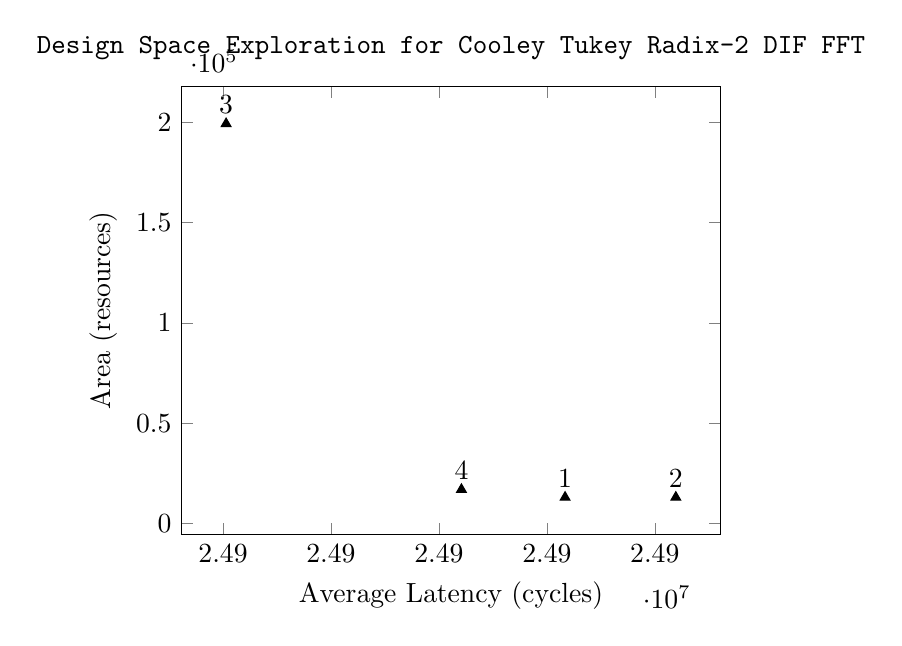
\begin{tikzpicture}
\label{graph:dse_CTfft}
\centering
	\begin{axis}[
		xlabel=Average Latency (cycles),
		ylabel=Area (resources),     
        nodes near coords, % Place nodes near each coordinate
    point meta=explicit symbolic, % The meta data used in the nodes is not explicitly provided and not numeric
	    title={\texttt{Design Space Exploration for Cooley Tukey Radix-2 DIF FFT}}]        
	\addplot[mark=triangle*, only marks, mark options={fill=black}] 
    table [% Provide data as a table
     meta index=2 % the meta data is found in the third column
     ] {
   x          y     label
24937082	13096    1
24937595	13098    2
24935512	199396   3
24936602	16984    4
	};
	\end{axis}
\end{tikzpicture}
\newline From the plot \ref{graph:dse_CTfft}, we see that solution 3 gives the best case latency. However, there are not enough LUTs in the target board to implement this design. Hence, optimizations of solution 4 are more appropriate for a practical best-case latency scenario. 
\newcolumntype{C}{>{\centering\arraybackslash}p{{0.25\linewidth}}}
\subsubsection{MachSuite FFT}
MachSuite is a collection of 19 diverse application benchmarks, which are high-level synthesizable. FFT algorithm which is one of the benchmark applications is explored to decide whether it meets our requirement.
\begin{table}[htbp]
\centering
\caption{Design Space Exploration for Machsuite FFT}
\label{tab:dse_machsuite}
\begin{tabular}{|m{2cm}|m{1.5cm}|m{3cm}|m{3cm}|}
\hline
\multicolumn{4}{|c|}{\textbf{Target: Avnet Zedboard Evaluation xc7z020clg484-1}} \\ \hline
\multicolumn{2}{|c|}{} & \textbf{Solution 1} & \textbf{Solution 2}\\ 
\hline
\multicolumn{2}{|c|}{\textbf{Optimization}} & \begin{tabular}[c]{@{}c@{}}Loop 0: Trip\\Count = 10,\\Loop 1: Trip\\Count = 1024\end{tabular} & \begin{tabular}[c]{@{}c@{}}Loops 1,2:\\Trip Count=512,\\Loop 3:\\Pipeline\end{tabular} \\ \hline
\multicolumn{2}{|c|}{\textbf{Estimated Clock Period}} & \makecell[c]{8.23} & \makecell[c]{8.23} \\ \hline
\multirow{2}{*}{\textbf{\begin{tabular}[c]{@{}c@{}}Latency\\ (cycles)\end{tabular}}} & \textbf{Min} & \makecell[c]{2170} & \makecell[c]{3195} \\ \cline{2-4} 
 & \textbf{Max} & \makecell[c]{49871994} & \makecell[c]{49871995} \\ \hline
\multirow{4}{*}{\textbf{\begin{tabular}[c]{@{}c@{}}Utilization\\ Estimates\end{tabular}}} & \textbf{BRAM\_18K} & \makecell[c]{0} & \makecell[c]{0} \\ \cline{2-4} 
 & \textbf{DSP48E} & \makecell[c]{56} & \makecell[c]{56} \\ \cline{2-4} 
 & \textbf{FF} & \makecell[c]{4511} & \makecell[c]{4513} \\ \cline{2-4} 
 & \textbf{LUT} & \makecell[c]{8529} & \makecell[c]{8529} \\ \hline
\end{tabular}
\end{table}

\subsubsection{Comparison of Execution Times}
\begin{table}[htbp]
\centering
\caption{Estimates of execution time in different FFT algorithms}
\label{tab:compare_fft}
\begin{tabular}{|m{0.2\linewidth}|m{0.25\linewidth}|m{0.25\linewidth}|m{0.25\linewidth}|}
\hline
 & \textbf{\makecell[c]{Non-recursive\\1-D FFT}} & \textbf{\makecell[c]{Radix-2\\DIF FFT}} &\textbf{MachSuite FFT}\\ \hline
\textbf{Best-case Execution Time} & 5387290 x 11.96 ns = 0.064 s & 1210 x 8.23 ns = 9.95 $\mu$s & 2170 X 8.23 ns = 17 $\mu$s \\ \hline
\end{tabular}
\end{table}

The execution time in Table \ref{tab:compare_fft} is calculated as the product of number of cycles and clock period. In Non-recursive 1-D FFT, execution time is of the order of a few milliseconds. As our application demands speed in the range of microseconds for gain over software implementation, Radix-2 FFT proves to be the optimal choice. \newline
\begin{adjustwidth}{2cm}{}
The ratio $R_{acceleration}$ = $\frac{t_{sw}}{t_{hw}}$ = $\frac{30.892}{9.95}$ = 3.1047\newline 
\end{adjustwidth} 
High-speed Streaming DMA Transfers from high performance ports of Zynq Processing system to Programmable logic via AXI Interface assure that the communication overhead is less. By using higher FPGA generations such as Virtex 7, a much higher speedup can be obtained and unroll factor increased. 
\chapter{Conclusion and Future Work}
\label{ch5_conclusion}
\section{Conclusion}
\label{6_1}
This report discussed the hardware acceleration by leveraging power-efficient heterogeneous architectures, namely GPUs and FPGAs by threaded programming (OpenCL) and high level synthesis. As the optimization objective was improving execution time, several compiler optimizations and platform-specific optimizations were used to inspect the gain in runtime. This report covered the study of two trending compute-intensive applications, isolation of software hot-spots, design decisions and improved implementation using heterogeneous hardware platform. Our experiments with MNIST digit classifier revealed that when the sequential C++ code is translated to parallel threads spawned together for concurrent execution, the speed-up is significant (as high as -- from our experiments). A huge dataset comprising of 10000 images was classified in a few microseconds. It also reveaved that any OpenCL compliant device, CPU or GPU, can offer acceleration depending on the number of low power cores available in the platform and also the memory access model. Hence, understanding of all the OpenCL models is crucial to schedule the work suitably among different compute units. The study of Fully Homomorphic Encryption scheme revealed that domain expertise is also a key factor to achieve hardware acceleration, in addition to accelerator-awareness. All computations performed in FHE are on ring lattices and hence, offloading the entire Bootstrapping logic onto hardware requires sound mathematical background on lattice-based computations. We noticed a gain of -- upon offloading the FFT to Zedboard. With high-end boards such as Virtex 7, a much higher speed-up can be accomplished and unrolling factor also increased, due to availability of more resources. The key challenge in hardware acceleration is ensuring that functionality is preserved upon offloading to an accelerator. High-speed Streaming DMA Transfers from high performance ports of Zynq Processing system to Programmable logic via AXI Interface assure that the communication overhead is less.
Explore assembly language FFT Libraries and study the speed-up.

\section{Future Work}
With the current choice of FPGA, a maximum of 2 FFT blocks can run in a single target board. Future works could incorporate:
\begin{itemize}
\item Identifying a novel way to \textbf{fit in a single AddToAccumulator block onto a single board}: \\The challenge in doing so is that each ciphertext comprises of an n-dimensional array (a[n]; n = 500) and an integer modulus b. Computations on ciphertexts take up alot of area and hence, these dimensions have to be intuitively handled.
\item \textbf{Reuse of the hardware FFT blocks in the new TFHE Library} implemented in April, 2017, to verify the generality of the implementation. As TFHE library already promises bootstrapping speed of less than 0.1 seconds, the gain in hardware for bootstrapping can be studied by porting specific "hot" functions to the hardware.
\item \textbf{Runtime analysis on coarse-grained and fine-grained Overlay Architectures} with efficient interfacing between host processor, DSP Units and other high-speed vector engines.
\end{itemize}

\begin{appendices}
	
\chapter{CNN}
\definecolor{highlight_red}{rgb}{1.0,0.92,0.8}
\definecolor{highlight_yellow}{rgb}{1.0,1.0,0.75}
\definecolor{highlight_green}{rgb}{0.75,1.0,0.75}
\newcommand{\Hilight}{\makebox[0pt][l]{\color{highlight_yellow}\rule[-4pt]{0.78\linewidth}{14pt}}}
\newcommand{\hl}{\makebox[0pt][l]{\color{highlight_red}\rule[-4pt]{0.18\linewidth}{12pt}}}
\newcommand{\hlg}{\makebox[0pt][l]{\color{highlight_green}\rule[-4pt]{0.3\linewidth}{12pt}}}

\lstset { %
	language=C,
	backgroundcolor=\color{white},
	basicstyle=\ttfamily\tiny,
	keywordstyle=\color{magenta}\ttfamily,
	stringstyle=\color{blue}\ttfamily,
	commentstyle=\color{darkgreen}\ttfamily,
    breakatwhitespace=false,
	breaklines=true,
    showstringspaces=false
}
\lstset{framesep=-5pt, xleftmargin=-5pt}
\begin{table}[!h]
\centering
\caption{Removal of Altera device-specific Macros}
\label{cnncode1:altera-dep-removal}
\begin{tabular}{l}
\toprule
\begin{lstlisting}[columns=fullflexible, language=C++, escapechar=\$]
void createDeviceBuffer() {
	cl_int status;
	cout << "Allocating buffers on the device memory" << endl;
	// data is allocated in BANK1 and weights are in BANK2 for efficient access.
	d_input_img = clCreateBuffer(context, CL_MEM_READ_ONLY |$\hl$ CL_MEM_BANK_1_ALTERA, 
		conv1.bot_shape->x * conv1.bot_shape->y  * conv1.bot_shape->z * sizeof(DTYPE), NULL, &status);
        conv1.d_input = clCreateBuffer(context, CL_MEM_WRITE_ONLY | $\hl$ CL_MEM_BANK_1_ALTERA,
		(conv1.bot_shape->x+2*conv1.pad) * (conv1.bot_shape->y+2*conv1.pad) * conv1.bot_shape->z * sizeof(DTYPE), NULL, &status);
        conv1.d_output = clCreateBuffer(context, CL_MEM_WRITE_ONLY | $\hl$ CL_MEM_BANK_1_ALTERA, 
		conv1.top_shape.x * conv1.top_shape.y  * conv1.top_shape.z * sizeof(DTYPE), NULL, &status);
	
	conv1.d_W = clCreateBuffer(context, CL_MEM_READ_ONLY | $\hl$ CL_MEM_BANK_2_ALTERA | CL_MEM_COPY_HOST_PTR, 
		conv1.K * conv1.K * conv1.bot_shape->z * conv1.top_shape.z * sizeof(WTYPE), conv1.W, &status);
	conv1.d_b = clCreateBuffer(context, CL_MEM_READ_ONLY | $\hl$ CL_MEM_BANK_2_ALTERA | CL_MEM_COPY_HOST_PTR, 
		conv1.top_shape.z * sizeof(WTYPE), conv1.b, &status);
        ........
}
\end{lstlisting}
\\
\bottomrule
\end{tabular}
\end{table}

\begin{table}[!h]
\centering
\caption{Loading kernel from Source}
\label{cnncode2:load-kernel-source}
\begin{tabular}{l}
\toprule
\begin{lstlisting}[columns=fullflexible, language=C++]
long LoadOpenCLKernel(char const* path, char **buf)
{
    FILE  *fp;
    size_t fsz;
    long   off_end;
    int    rc;
    /* Open the file */
    fp = fopen(path, "r");
    if( NULL == fp ) {
        return -1L;
    }
    /* Seek to the end of the file */
    rc = fseek(fp, 0L, SEEK_END);
    if( 0 != rc ) {
        return -1L;
    }
    /* Byte offset to the end of the file (size) */
    if( 0 > (off_end = ftell(fp)) ) {
        return -1L;
    }
    fsz = (size_t)off_end;
    /* Allocate a buffer to hold the whole file */
    *buf = (char *) malloc( fsz+1);
    if( NULL == *buf ) {
        return -1L;
    }
    /* Rewind file pointer to start of file */
    rewind(fp);
    /* Slurp file into buffer */
    if( fsz != fread(*buf, 1, fsz, fp) ) {
        free(*buf);
        return -1L;
    }
    /* Close the file */
    if( EOF == fclose(fp) ) {
        free(*buf);
        return -1L;
    }
    /* Make sure the buffer is NUL-terminated, just in case */
    (*buf)[fsz] = '\0';
    /* Return the file size */
    return (long)fsz;
}
\end{lstlisting}
\\
\bottomrule
\end{tabular}
\end{table}

\begin{table}[!h]
\centering
\caption{Initialization of OpenCL Objects for Altera FPGA (Taken from Altera Design Examples)}
\label{cnncode3:altera-opencl-init}
\begin{tabular}{l}
\toprule
\begin{lstlisting}[columns=fullflexible, language=C++, escapechar=\$]
bool init_opencl() {
	cl_int status;	
	printf("Initializing OpenCL\n");
	if(!setCwdToExeDir()) {
	  return false;
	}	
	// Get the OpenCL platform.
	$\Hilight$ platform = findPlatform("Altera");
	 if(platform == NULL) {
	  printf("ERROR: Unable to find Altera OpenCL platform.\n");
	 return false;
	}	
	// Query the available OpenCL device.
	$\Hilight$ devices.reset(getDevices(platform, CL_DEVICE_TYPE_ALL, &num_devices));
	printf("Platform: %s\n", getPlatformName(platform).c_str());
	printf("Found %d devices in the board. Using only one device for this app\n", num_devices);
	for(unsigned i = 0; i < num_devices; ++i) {
	  printf("  %s\n", getDeviceName(devices[i]).c_str());
	}
	$\Hilight$ target_device = devices[0];	
	// Create the context.
	context = clCreateContext(NULL, num_devices, &target_device, &oclContextCallback, NULL, &status);
	checkError(status, "Failed to create context");
	
	std::string binary_file = getBoardBinaryFile("cnn_kernels", target_device);
	printf("Using AOCX: %s\n", binary_file.c_str());
	$\Hilight$ program = createProgramFromBinary(context, binary_file.c_str(), &target_device, num_devices);
	
	// Build the program that was just created.
	status = clBuildProgram(program, 0, NULL, "", NULL, NULL);
	checkError(status, "Failed to build program");
	
	kernel.reset(num_kernels);
	
	// Command queue.
	queue = clCreateCommandQueue(context, target_device, CL_QUEUE_PROFILING_ENABLE, &status);
	checkError(status, "Failed to create command queue");
	
	// Kernel.
	kernel[0] = clCreateKernel(program, "filter3D", &status);
	checkError(status, "Failed to create kernel");
	kernel[1] = clCreateKernel(program, "maxpool3D", &status);
	checkError(status, "Failed to create kernel");
	kernel[2] = clCreateKernel(program, "iplayer", &status);
	checkError(status, "Failed to create kernel");
	kernel[3] = clCreateKernel(program, "relu_layer", &status);
	checkError(status, "Failed to create kernel");
	kernel[4] = clCreateKernel(program, "softmax", &status);
	checkError(status, "Failed to create kernel");

	return true;
}
\end{lstlisting}
\\
\bottomrule
\end{tabular}
\end{table}

\begin{table}[!h]
\centering
\caption{Initialization of OpenCL Objects for a GPU Device}
\label{cnncode4:gpu-opencl-init}
\begin{tabular}{l}
\toprule
\begin{lstlisting}[columns=fullflexible, language=C++,escapechar=\$]
bool init_opencl() {
	cl_int status;
	int err;
	cl_platform_id platform_ids[5];		
	char *KernelSource;
	long lFileSize;
	cl_uint dev_cnt = 0;

        printf("Initializing OpenCL\n");
	clGetPlatformIDs(0, 0, &dev_cnt);
	$\Hilight$ clGetPlatformIDs(dev_cnt, platform_ids, NULL);
        int gpu = 1;
	for(unsigned i = 0;i < dev_cnt; i++)
	{
	   err = clGetDeviceIDs(platform_ids[i], $\hlg$ gpu ? CL_DEVICE_TYPE_GPU:CL_DEVICE_TYPE_CPU, 1, &target_device, NULL);
           if(err == CL_SUCCESS)
           {
		break;
	   }
        }
	if (err != CL_SUCCESS)
	{
	   printf("Error: Failed to create a device group!\n");
	   return EXIT_FAILURE;
   	}

	// Create the context.
        context = clCreateContext(0, 1, &target_device, NULL, NULL, &err);
	if (!context)
	{
	    printf("Error: Failed to create a compute context!\n");
	    return EXIT_FAILURE;
	}

	$\Hilight$ lFileSize = LoadOpenCLKernel("device/cnn_kernels.cl", &KernelSource);
	if( lFileSize < 0L ) {
		perror("File read failed");
		return 1;
	}

	$\Hilight$ program = clCreateProgramWithSource(context, 1, (const char **) & KernelSource, NULL, &err);
	if (!program)
	{
		printf("Error: Failed to create compute program!\n");
		return EXIT_FAILURE;
	}

	// Build the program that was just created.
	$\Hilight$ status = clBuildProgram(program, 0, NULL, "", NULL, NULL);
	checkError(status, "Failed to build program");
	
	kernel.reset(num_kernels);
	// Command queue.
	$\Hilight$ queue = clCreateCommandQueue(context, target_device, CL_QUEUE_PROFILING_ENABLE, &status); 
	checkError(status, "Failed to create command queue");
	
	// Kernel.
	kernel[0] = clCreateKernel(program, "filter3D", &status);
	checkError(status, "Failed to create kernel");
	kernel[1] = clCreateKernel(program, "maxpool3D", &status);
	checkError(status, "Failed to create kernel");
	kernel[2] = clCreateKernel(program, "iplayer", &status);
	checkError(status, "Failed to create kernel");
	kernel[3] = clCreateKernel(program, "relu_layer", &status);
	checkError(status, "Failed to create kernel");
	kernel[4] = clCreateKernel(program, "softmax", &status);
	checkError(status, "Failed to create kernel");
	return true;
}
\end{lstlisting}
\\
\bottomrule
\end{tabular}
\end{table}
	
\chapter{FHEW}
\begin{table}[!h]
\centering
\caption{AXI-Stream Input-Output data handler}
\label{fhewcode1:fft_stream}
\begin{tabular}{l}
\toprule
\begin{lstlisting}[columns=fullflexible, language=C++,escapechar=\$]
#include <hls_video.h> //for streaming data
#include <ap_axi_sdata.h> //for defining channel attributes
typedef ap_axiu<64,1,1,1> IOchannel; // <data, user, ID, destination>

void handleFFT(hls::stream<IOchannel> &inStream, hls::stream<IOchannel> &outStream)
{
#pragma HLS INTERFACE axis port=inStream
#pragma HLS INTERFACE axis port=outStream
    IOchannel inChannel, outChannel;
    complex_t input[2*N], output[N];
    int idx;
    for(idx = 0; idx < 2*N; idx++)
    {
    #pragma HLS PIPELINE
        //Read and Cache Input channel value once (Block here if FIFO sender is empty)
        inChannel = inStream.read();
        input[idx].re = *((double*) (&inChannel.data));
        inChannel = inStream.read();
        input[idx].im = *((double*) (&inChannel.data));
    }
    FFT(input, output);
    outChannel.keep = inChannel.keep;
    outChannel.strb = inChannel.strb;
    outChannel.user = inChannel.user;
    outChannel.id   = inChannel.id;
    outChannel.dest = inChannel.dest;
    outChannel.last = 0;

    for(idx = 0; idx < N-1; idx++)
    {
		outChannel.data = *((ap_uint<64> *)(&output[idx].re));
		outStream.write(outChannel); //Reference: Vivado Design Suite User Guide
		outChannel.data = *((ap_uint<64> *)(&output[idx].im));
		outStream.write(outChannel);
    }
    outChannel.data = *((ap_uint<64> *)(&output[idx].re));
    outStream.write(outChannel);
    outChannel.data = *((ap_uint<64> *)(&output[idx].im));
    outStream.write(outChannel);
    outChannel.last = 1;
}
\end{lstlisting}
\\
\bottomrule
\end{tabular}
\end{table}

\begin{table}[!h]
\centering
\caption{Non-recursive 1-D FFT}
\label{fhewcode2:fft1}
\begin{tabular}{l}
\toprule
\begin{lstlisting}[columns=fullflexible, language=C++,escapechar=\$]
#include "fft.h"
#include <stdio.h>
#include <stdlib.h>
#include <math.h>
#include <complex>

#define PI 3.1415926535897932384626434
#define N 1024
typedef struct complex_t {
    double re;
    double im;
} complex_t;

void FFT(complex_t input[2*N], complex_t output[N])
{
    int k, n;
    complex_t mul_res, conv_res, add_res;
    // Compute N DFTs of length 1 using naive method
    FFT_label0:for (k = 0; k < N; k++)
    {
       conv_res.re = 1;
       conv_res.im = 0; // -2*PI*n*k2/N2 --> k2 = 0, n = 0 for 1D Convolution
       multiply(input[k], conv_res, &mul_res);
       /* Multiply by the twiddle factors  ( e^(-2*pi*j/N * k1*k2)) and transpose
          conv_from_polar(1, -2.0*PI*k1*k2/N, &conv_res); --> k2 = 0 for 1D Convolution */
       multiply(conv_res, mul_res, &mul_res);
       input[k] = mul_res;
    }

    for(k = 0; k < N; k++)
    {
       output[k].re = 0.0;
       output[k].im = 0.0;
       FFT_label2:for(n = 0; n < N; n++)
       {
    	  std::complex<double> t = std::polar(1.0, -2 * PI * n* k / N);
    	  conv_res.re = std::real(t);
    	  conv_res.im = std::imag(t);
          multiply(input[n], conv_res, &mul_res);
          add(output[k], mul_res, &add_res);
          output[k] = add_res;
       }
    }
 }
//-------------------Utility Functions-------------------------
 void add(complex_t left, complex_t right, complex_t* result)
 {
    (*result).re = left.re + right.re;
    (*result).im = left.im + right.im;
 }

 void multiply(complex_t left, complex_t right, complex_t* result)
 {
    (*result).re = left.re*right.re - left.im*right.im;
    (*result).im = left.re*right.im + left.im*right.re;
 }
\end{lstlisting}
\\
\bottomrule
\end{tabular}
\end{table}

\begin{table}[!h]
\centering
\caption{Radix-2 DIF FFT}
\label{fhewcode3:CTfft}
\begin{tabular}{l}
\toprule
\begin{lstlisting}[columns=fullflexible, language=C++,escapechar=\$]
void fft(Complex x[2*N])
{
	unsigned int k = N, n;
	double thetaT = 3.14159265358979323846264338328L / N;
	Complex phiT = Complex(cos(thetaT), sin(thetaT)), T;

	fft_label0:for(unsigned int i=0; i < 10; i++) 
//because 2^10 = 1024 - After 9 right shifts, k becomes <= 1 => 2^0 = 1
	{
		n = k;
		k >>= 1;
		phiT = phiT * phiT;
		T = 1.0L;
		fft_label1:for (unsigned int l = 0; l < k; l++)
		{
			fft_label2:for (unsigned int a = l; a < N; a += n)
			{
				unsigned int b = a + k;
				Complex t = x[a] - x[b];
				x[a] = x[a] + x[b];
				x[b] = t * T;
			}
			T *= phiT;
		}
	}

	// Decimate
	unsigned int m = (unsigned int)log2(N);
	fft_label3:for (unsigned int a = 0; a < N; a++)
	{
		unsigned int b = a;
		// Reverse bits
		b = (((b & 0xaaaaaaaa) >> 1) | ((b & 0x55555555) << 1));
		b = (((b & 0xcccccccc) >> 2) | ((b & 0x33333333) << 2));
		b = (((b & 0xf0f0f0f0) >> 4) | ((b & 0x0f0f0f0f) << 4));
		b = (((b & 0xff00ff00) >> 8) | ((b & 0x00ff00ff) << 8));
		b = ((b >> 16) | (b << 16)) >> (32 - m);
		if (b > a)
		{
			Complex t = x[a];
			x[a] = x[b];
			x[b] = t;
		}
	}
}
\end{lstlisting}
\\
\bottomrule
\end{tabular}
\end{table}
\end{appendices}

\bibliographystyle{unsrt}
\bibliography{content/references.bib}

\end{document}
